
\documentclass{acm_proc_article-sp-sigmod09}

\usepackage{graphicx} 
\usepackage[english]{babel}
\usepackage{cleveref}
\usepackage{float}
\usepackage{subfig}
\usepackage{url}
\usepackage[htt]{hyphenat}

\begin{document}

%
% --- Author Metadata here ---
%\conferenceinfo{ACM SIGMOD}{'09 Providence, RI, USA}
%\setpagenumber{50}
%\CopyrightYear{2002} % Allows default copyright year (2002) to be over-ridden - IF NEED BE.
%\crdata{0-12345-67-8/90/01}  % Allows default copyright data (X-XXXXX-XX-X/XX/XX) to be over-ridden.
% --- End of Author Metadata ---

\title{Understanding the NYC Taxi Service}

\numberofauthors{3}

\author{
	Willi Menapace\\
	\texttt{203778}\\
	\texttt{willi.menapace@studenti.unitn.it}
	\and
	Luca Zanella\\
	\texttt{207520}\\
	\texttt{luca.zanella-3@studenti.unitn.it}
	\and
	Daniele Giuliani\\
	\texttt{203508}\\
	\texttt{daniele.giuliani@studenti.unitn.it}
}





\maketitle
\begin{abstract}
	
Big Data is rapidly becoming a predominant field in ICT. Its importance is continuously growing due to the huge volume and variety of available data. In this work we try to exploit its descriptive and predictive power in order to better comprehend the evolution and current state of the taxi service in New York City, leveraging the service data that the NYC Taxi and Limousine Commission (TLC) made publicly available.

We analyze a wide spectrum of views, starting with a general overview of the service evolution in time and confronting it with with the emerging phenomenon of ride-hailing applications such as Uber, Juno and Lyft. We then proceed to perform a segmentation of the traffic in order to understand better the characterization of taxi customers and later continue by analyzing subjects such as movement patterns of traffic, competition between yellow and green taxis and characteristics of airport traffic.

The results we present should help the reader understand the main trends and characteristics of the taxi service, which may suggest ways to increase the quality and popularity of the service.

\end{abstract}

\section{Introduction}
The NYC Taxi and Limousine Commission (TLC) has publicly made available a dataset containing data about taxi trips performed in New York from January 2009 to June 2018. This study aims at exploiting this dataset to understand how the New York taxi service works.

The report describes step by step how our analysis is performed. It starts from data acquisition, compression, transformation and cleaning and then proceeds analyzing different aspects of the data in order to provide the reader with an overview of how the taxi service in New York works.

The main technology enabling the analysis of such dataset is Apache Spark, coupled with R for data visualization.

\section{Data Acquisition and compression}

The main dataset used for the analysis is publicly available at \url{http://www.nyc.gov/html/tlc/html/about/trip_record_data.shtml}. We download the data for the time period from January 2010 to June 2018, both for Yellow and Green taxis which consists of ~200GB of comma separated value files containing over a 1 Billion records. The schema of the dataset varies by year and taxi company for a total of 6 different schemas. The main columns available through the datasets refer to pickup and dropoff datetimes, trip distance, number of passengers, fare amount, total amount, tip amount, extras and taxes, tolls, ratecode and payment type. The most notable difference between the data is the information about pickup and dropoff locations which is expressed with latitutes and longitudes until 2016 and with numerical taxi zone identifiers for the following years.

After acquisition of the data we proceed to compress it to .tar.gz format in order to handle them more effectively. The compression is significant, with a resulting dataset size of 43GB. The gzip format however is not particularly suited for big data analysis. The parquet file format provides significant performance advantages such as columnar storage, which allows computations that only need specific columns to access them selectively, specific compression algorithms for each column with dictionary specific encodings and the possibility to decode the file even partially, which is convenient in distributed environments such as Spark. The size of the dataset is slightly reduced to 39GB.

\section{Data transformation}

The parquet dataset is then transformed into a common schema format to uniform the data and ease the analysis. We decide to adopt the following schema:

\begin{itemize}
	\item \path{taxi_company}, ``green'' or ``yellow'' according to the taxi type that served the trip
	\item \path{pickup_datetime}, date and time of the pickup
	\item \path{dropoff_datetime}, date and time of the dropoff
	\item \path{pickup_location_id}, taxi zone id where the pickup happened, -1 if the zone is unknown
	\item \path{dropoff_location_id}, taxi zone id where the dropoff happened, -1 if the zone is unknown
	\item \path{passenger_count}, number of passengers onboard
	\item \path{trip_distance}, the metered distance in miles
	\item \path{ratecode_id}, the fare rate used for the calculation of the amount, which includes special rates for JFK or Newark trips.
	\item \path{fare_amount}, the fare amount for the trip in \$
	\item \path{tolls_amount}, the amount of tolls in \$
	\item \path{total_amount}, the total amount for the trip in \$. It includes tips only for credit card payments.
	\item \path{mta_tax}, the amount due to MTA tax in \$
	\item \path{improvement_surcharge}, the amount due to the improvement surcharge in \$
	\item \path{extra}, the amount due to extra in \$ including only rush hour and overnight charges
	\item \path{tip_amount}, the tip amount in \$. It is set only for credit card payments
	\item \path{payment_type}, the used payment method
\end{itemize}

Note that the common schema codifies the pickup and dropoff locations as the ids of the zone where the pickup or the dropoff happened and not as coordinates. The main challenge for schema conversion is the transformation of dropoff and pickup locations expressed as coordinates into the respective taxi zones. The dataset is accompanied by a shapefile which specifies the geographical boundaries of each zone. Unfortunately, naive algorithms for dataset conversion directly using the shapefile are able to only convert some tens of records per second per processor which would make the conversion of 1 Billion of records unfeasible. Instead, we decide to develop a more efficient algorithm for zone association which makes use of look up tables to increase the performance of the conversion up to the thousands of records per second, allowing the complete conversion of the dataset.

\subsection{Coordinates to Zone conversion algorithm}

Until 2016, information about pickup and dropoff locations is represented through latitudes and longitudes expressed in the World Geodetic System (WGS) coordinate system. The need to have a consistent schema through the years lead us to develop an efficient algorithm to convert the information about pickup and dropoff locations to numerical taxi zone identifiers. 

According to the shapefile provided with the dataset, the city of New York is divided in 265 zones and the geometric locations, representing each of these zones, are expressed through the NAD83 / New York Long Island (ftUS) coordinate reference system. Our first attempt is to divide New York in a 1000x1000 lookup matrix in which each tile is delimited by some coordinates and is associated with a list of possible zones which are present in these boundaries in order to restrict the search. This is achieved by including each shape record, representing a specific zone of New York, in the tiles forming the smallest rectangle surrounding that zone. Due to this coarse approximation, each tile may contain many zones.

Given the latitude and the longitude of a location in the correct coordinate system, the numerical taxi zone identifier can be obtained by looking at the corresponding tile inside the lookup matrix, scanning each contained shape and retrieving the shape record containing that point. This algorithm is a notable improvement over the naive method, being able to convert some hundreds of records per second for each processor, but still does not allow for the conversion of the whole dataset. The main problem is the need to still linearly search through a list of shapes, although its average length is considerably reduced with respect to the naive implementation. The optimization that allows us to reach the target performance is to refine the coarse list of possible zones for each tile until the point where we directly associate each matrix tile with a unique zone id instead of a list of possible zones. This is possible because by using a 1000x1000 lookup matrix, each tile corresponds to a rectangular region of circa 70x70m, which is granular enough to be associated with a single zone even in the case where it lies across zone boundaries. This zone refinement is achieved by defining a set of probing points, such as the ones represented in fig. \ref{fig:probingPoints}, and checking which zones in the coarse list for the current tile actually contain at least one of the probing points. Whenever a tile is associated with more than one zone even with this refinement, we randomly choose only one for performance reasons. Due to the high matrix granularity, this situation occurs in a minority of regions and when it happens it causes tolerable approximations. The performance achieved through this optimization allows for the conversion of roughly 4000 records per core per second, which makes it possible for an 8 thread processor to convert the whole dataset overnight.

The dataset in common format for years 2010 to 2018 resulting from the conversion has a size of 24GB.

\begin{figure}
	\centering
	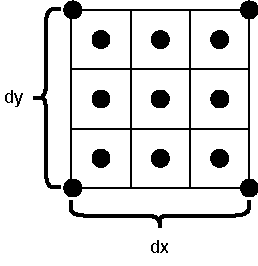
\includegraphics{resources/probing_points.pdf}
	\caption{The probing points for a single tile used for checking which zones are actually contained in it. dx and dy, the width and height of each tile, correspond to approximately 70m.}
	\label{fig:probingPoints}
\end{figure}

\section{Data cleaning}

An analysis of the dataset in the common format highlights data quality problems in some of its entries. To increase the quality of the analysis we decide to perform some data cleaning on the dataset.
Null entries are a minority of the dataset, so we decide to drop every entry in the dataset with a null attribute. Every categorical feature is then enforced to assume a value in its set of legal values. In particular, location ids are enforced to be valid ids and each entry for which our coordinate conversion algorithm was not able to identify a correspondent taxi zone is dropped. We then plot the distribution of the values of each numerical feature and conservatively identify a point in its tail after which all entries are dropped, for example tolls amounts greater than 120\$ are discarded because very irrealistic according to the distribution of the tolls and probably symptom of poor data quality. We also conservatively drop entries for which the duration is greater than 24 hours or for which the year is not in the range from 2010 to 2018.

The resulting dataset contains 1.07 Billion entries versus the original 1.38 Billion entries and the size of the dataset reduced to 20GB.

\section{Preliminary analysis}
\label{sec:preliminaryAnalysis}
The first phase of the analysis is the study of the domain. The New York taxi service is operated by private individuals owning taxi licenses. Two kind of taxi cabs are present, each one with specific characteristics and limitations: yellow cabs, also called medallion taxis, and green cabs, also called boro taxis. The city of New York is divided in five different districts called boroughs, shown in \cref{fig:boroughsMap}: Manhattan, Bronx, Brooklyn, Queens and Staten Island and each one is further divided into taxi zones. Both yellow and green taxis share the same fare system, but, while yellow cabs are allowed to pickup passengers anywhere in the five boroughs, green cabs are not allowed to pick up passengers in South Manhattan, LaGuardia Airport and JFK Airport, the most profitable zones for yellow taxis, but are allowed to drop the passengers anywhere. The reasons for the limitations of green taxis are two. The first is that before the introduction of green taxis, finding a cab in the boroughs outside Manhattan was challenging because yellow taxis prefer to stay in the more profitable Manhattan zone, so this limitation favors the distribution of taxis in the outer zones. The second reason is that the introduction of new licenses for green taxis was seen as a menace from the yellow cab business which strongly opposed to their introduction and obtained that green taxis would not be allowed to pick up passengers at the lucrative LaGuardia and JFK airport zones, with the exception of previously arranged trips by passengers with the driver.

\begin{figure}
	\centering
	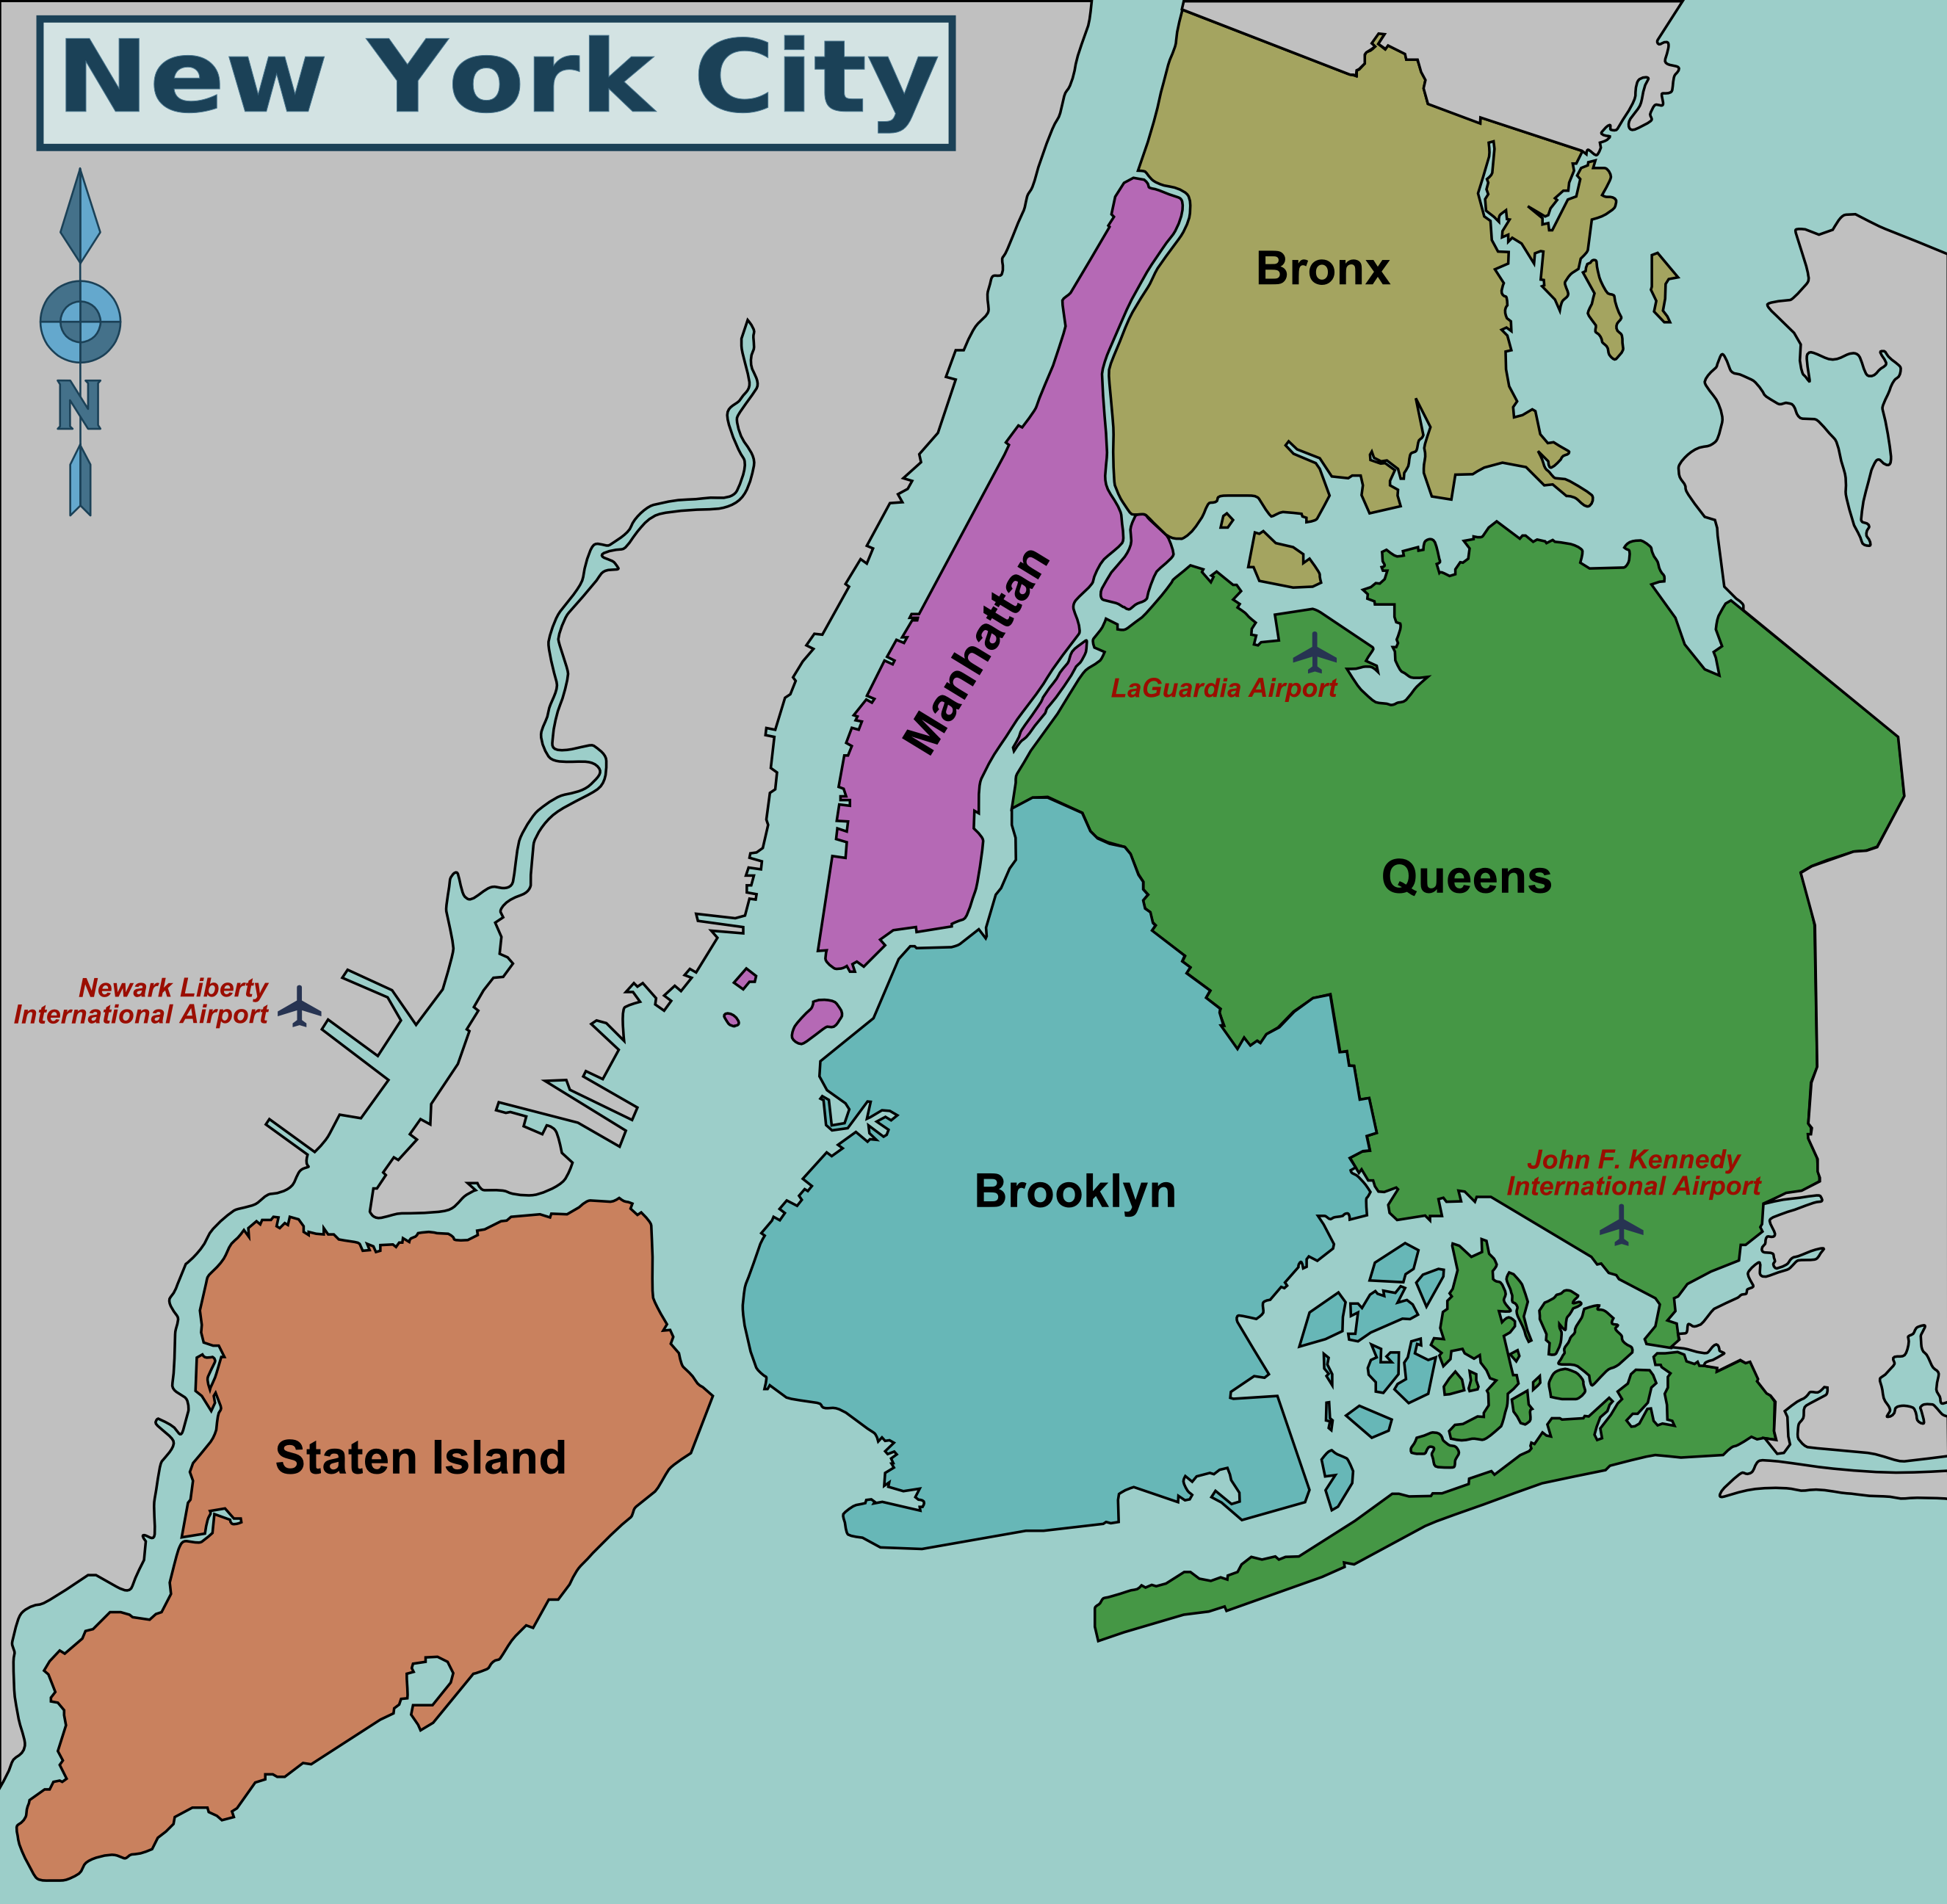
\includegraphics[width=1\columnwidth]{resources/nyc_borough_map.png}
	\caption{The five boroughs of New York. Notice the position of the three airports: LaGuardia, JFK and Newark. Courtesy of https://nycmap360.com}
	\label{fig:boroughsMap}
\end{figure}

The fare system is shared by both yellow and green cabs. The amount starts from a base of 2.50\$ and increases as a function of time when moving slowly and as a function of distance when moving faster. Some extras may be added based on the hour of the day as well as various taxes. The passenger is also requested to pay for any incurred toll and is requested to tip the driver with a variable amount that ranges around 20\% of the total. Fares between any zone of Manhattan and LaGuardia airport have a special flat rate of 52\$ plus extras. Newark airport also has a special rate which adds a 17.50\$ surcharge.

\begin{figure}
	\centering
	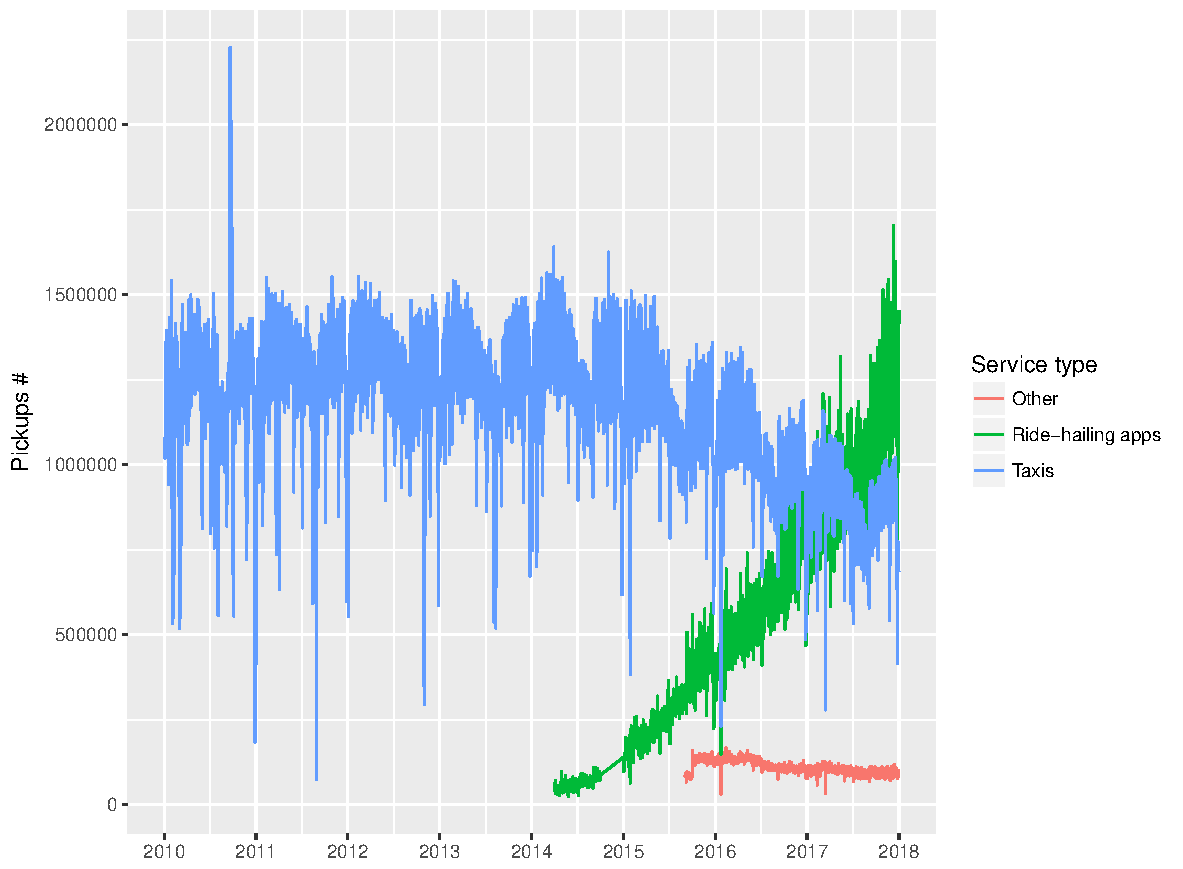
\includegraphics[width=1\columnwidth]{resources/fhv_vs_taxi.pdf}
	\caption{Historical taxi and ride hailing apps activity. Data from https://github.com/toddwschneider/nyc-taxi-data}
	\label{fig:uberVsTaxis}
\end{figure}

The analysis starts with a high level, exploration of the data. As shown in \cref{fig:travelsByYear} the number of total trips performed in the years grows slightly until 2015 and decreases in the following years. Note immediately that 2010 and 2016 are anomalous years due to data quality problems that caused the removal of entire months of entries for those year. Looking at the profits, calculated based on the total amount, we can see an increasing trend in the years until 2015, after which there is a drop in the profits because of the reduced number of trips performed by the taxis. The growth of the profits, despite the only slight increase of the number of trips is given by a higher cost per trip in the years, as shown in \cref{fig:travelsByYear}. The decline of the number of taxi trips started in 2015 can be explained by the growth in popularity of ride hailing services such as Uber, Lyft and Juno which, from 2015, are becoming widespread in the city as shown in \cref{fig:uberVsTaxis} and in 2017 surpassed taxis in popularity.

\begin{figure}
	\centering
	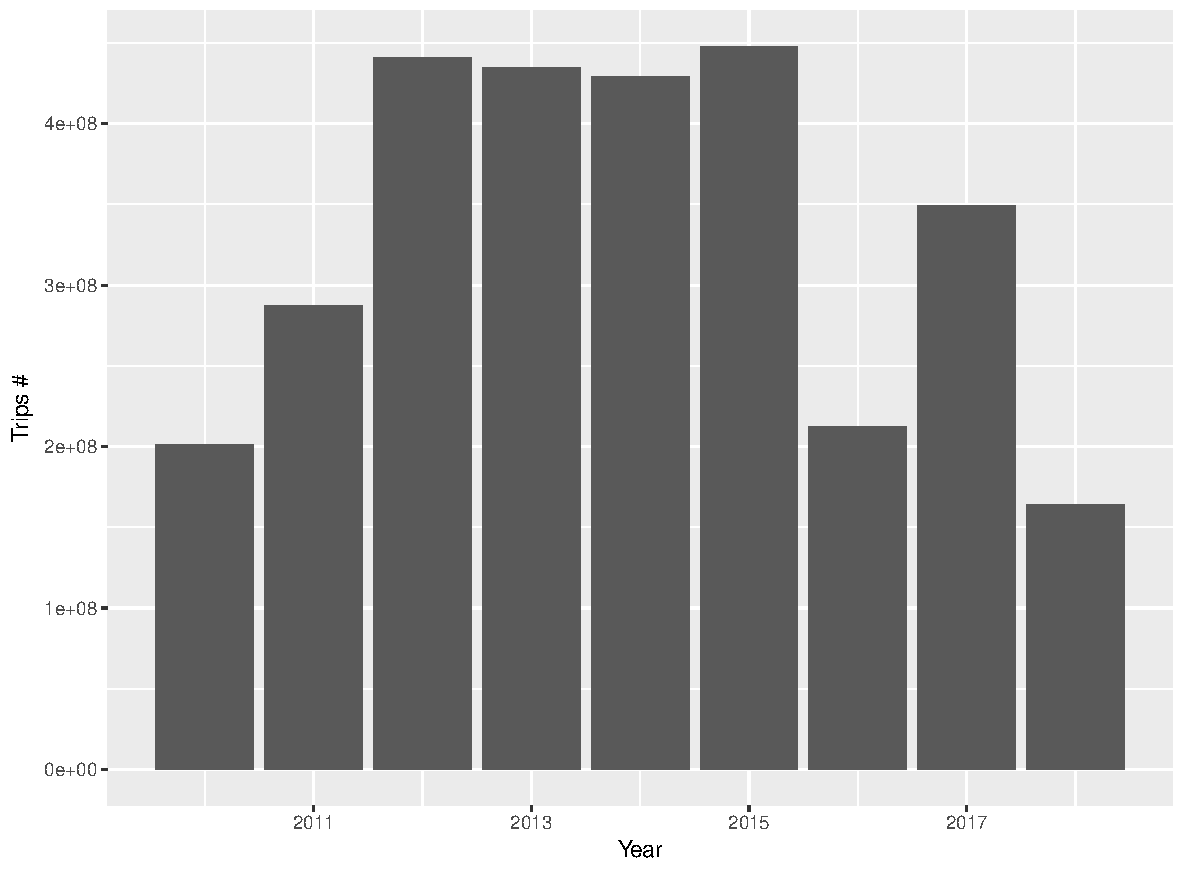
\includegraphics[width=1\columnwidth]{resources/base_plots/travels_by_year.pdf}
	\caption{Total trips performed each year. Data for years 2010 and 2016 is missing due to data quality problems, while data for 2018 is only relative for the period January-June. Notice the decrease started in 2015.}
	\label{fig:travelsByYear}
\end{figure}

\begin{figure}
	\centering
	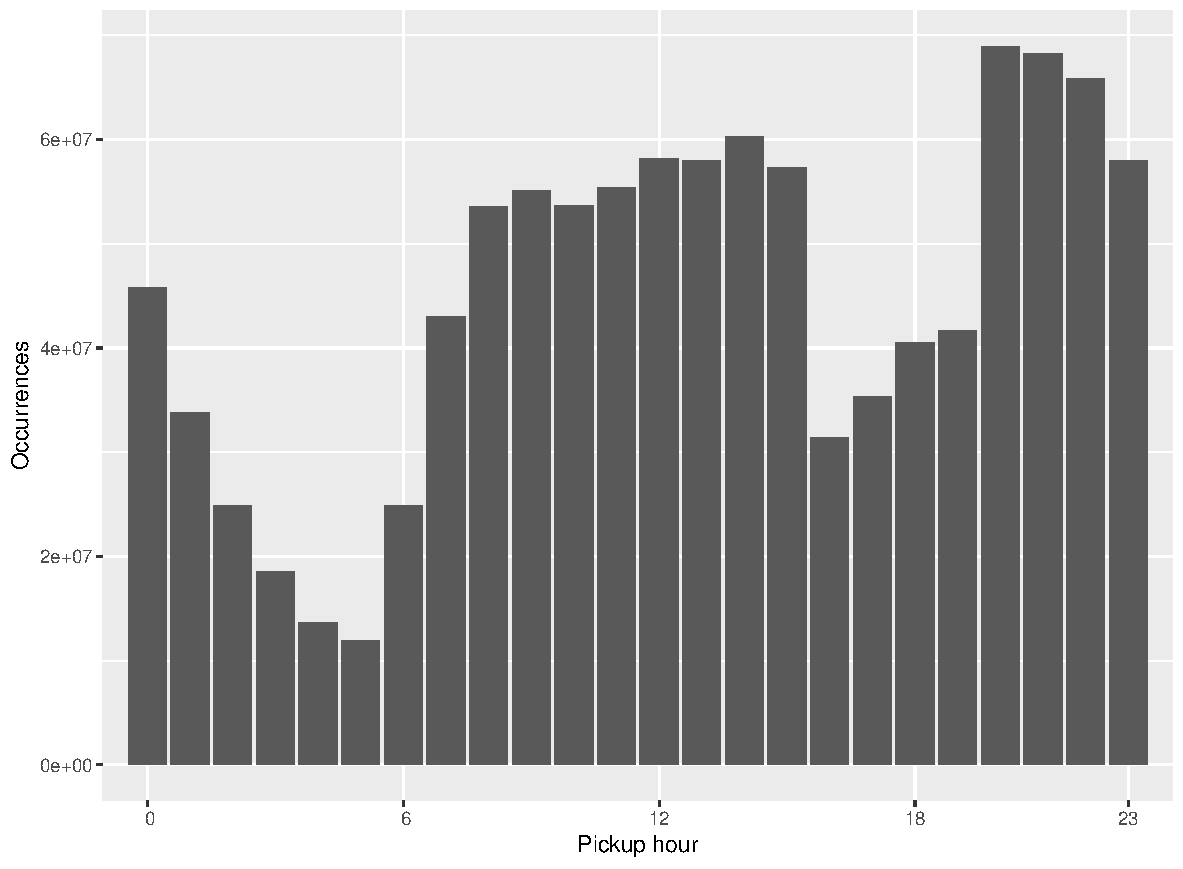
\includegraphics[width=1\columnwidth]{resources/base_plots/pickup_hour_dist.pdf}
	\caption{Number of pickups as a function of the pickup hour. Notice the major activity periods at 8-16 and 20-24.}
	\label{fig:pickupHourDist}
\end{figure}

\begin{figure}
	\centering
	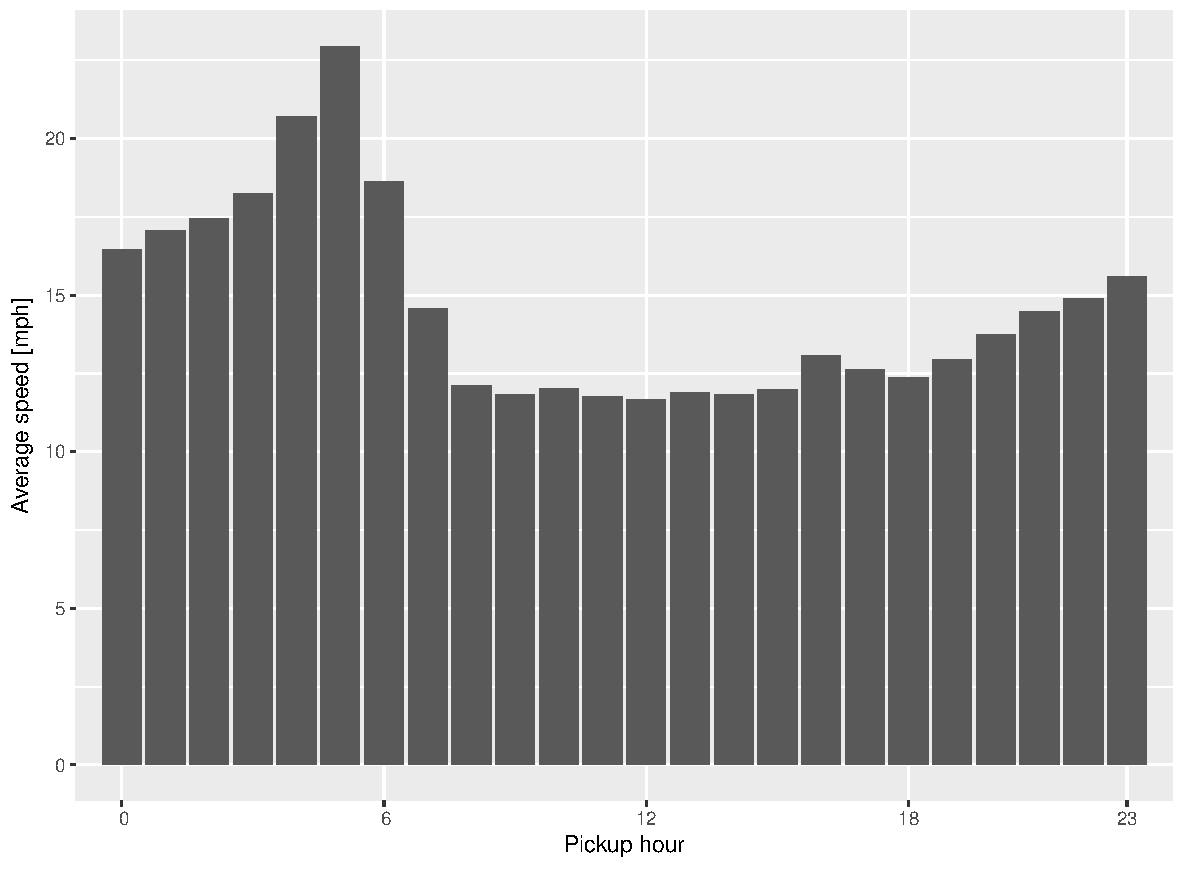
\includegraphics[width=1\columnwidth]{resources/base_plots/avg_speed_by_pickup_hour_dist.pdf}
	\caption{Average speed as a function of pickup hour. Notice how the average speed increases in the periods of minor activity.}
	\label{fig:speedByHour}
\end{figure}

\begin{figure}
	\centering
	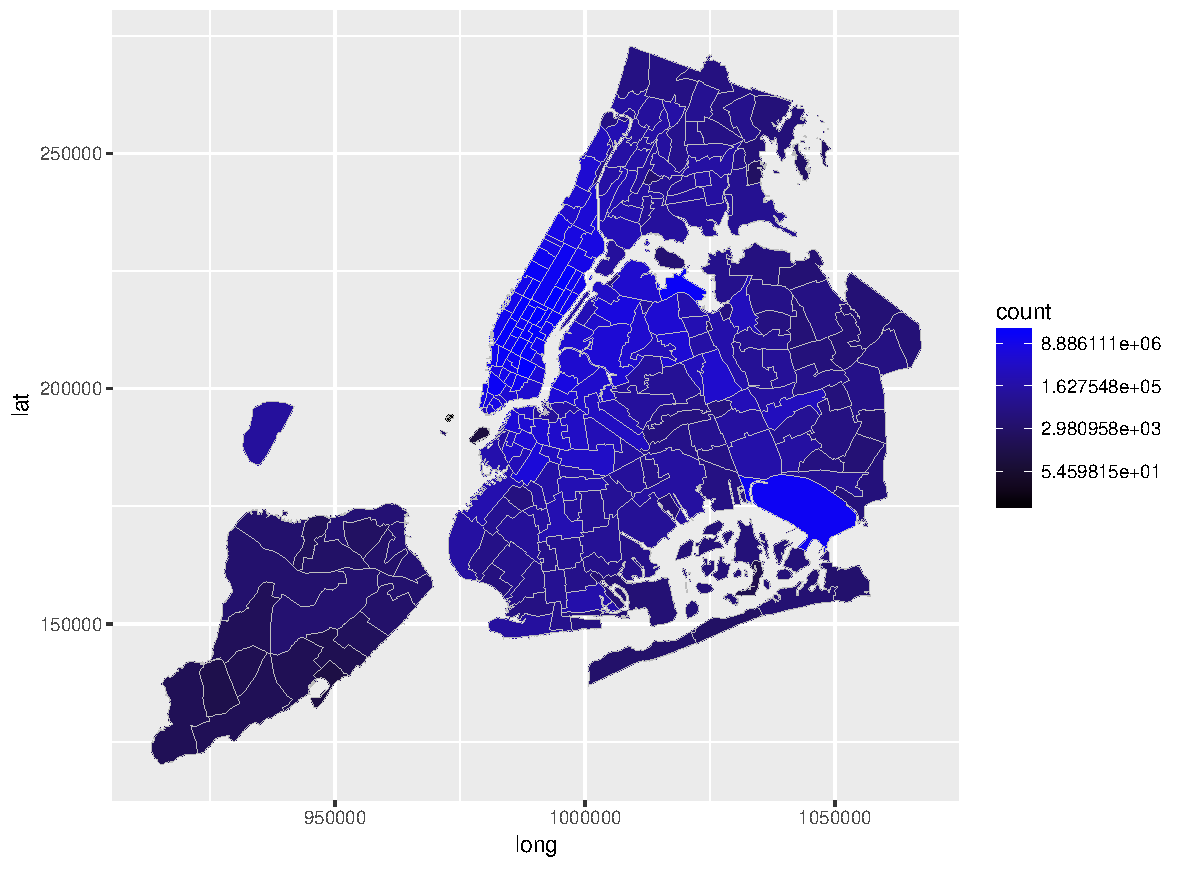
\includegraphics[width=1\columnwidth]{resources/base_plots/pickup_location_id_dist_map.pdf}
	\caption{Map in logarithmic scale showing the number of pickups per zone. Dropoff location map is omitted because of close similarity.}
	\label{fig:pickupDistributionMap}
\end{figure}

\begin{figure}
	\centering
	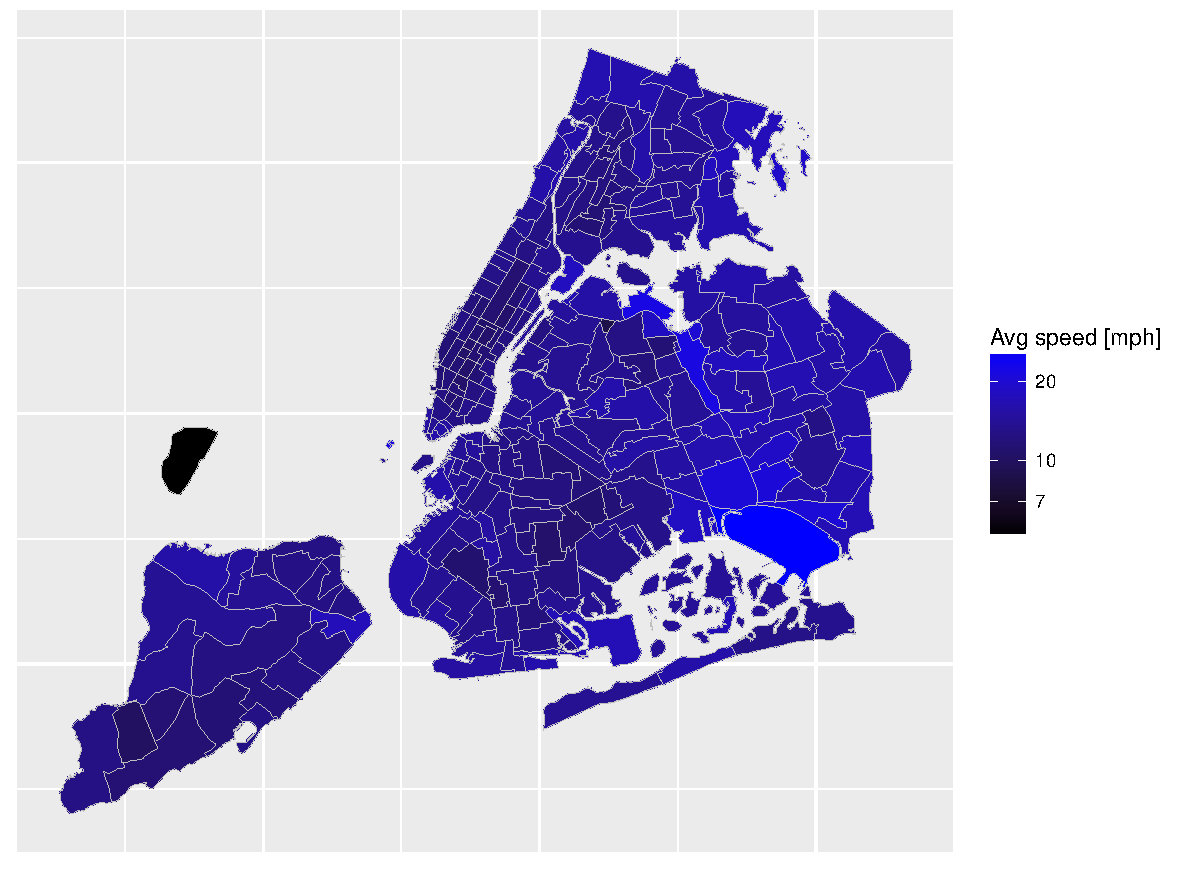
\includegraphics[width=1\columnwidth]{resources/base_plots/avg_speed_by_pickup_location_map.pdf}
	\caption{Map showing the average speed per pickup zone. Notice how outer boroughs typically feature higher average speeds, an indicator of the quantity of traffic.}
	\label{fig:speedMap}
\end{figure}

\begin{figure}
	\centering
	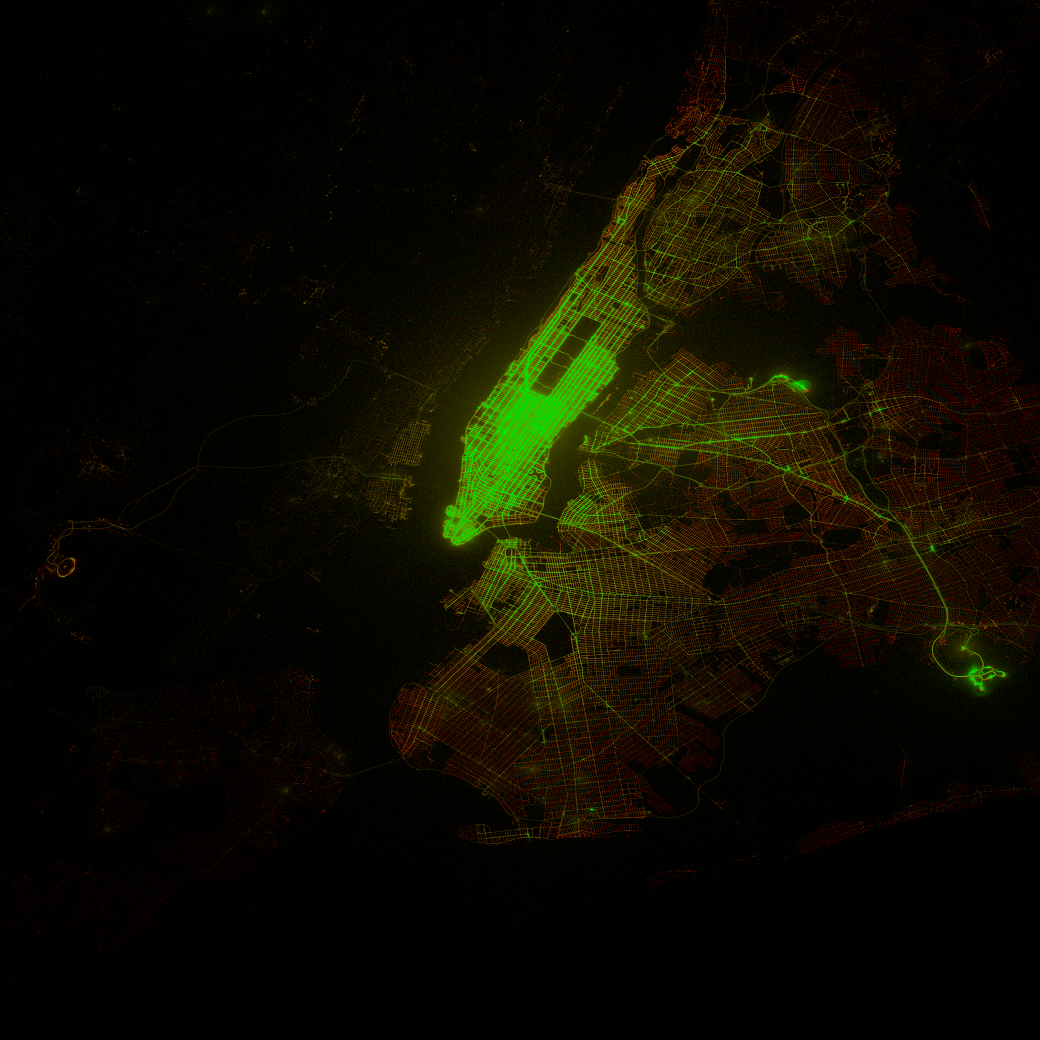
\includegraphics[width=1\columnwidth]{resources/base_plots/pickup_vs_dropoff.png}
	\caption{Map showing pickups points in green and dropoff points in red. Notice how dropoff points are granularly distributed across every street, while pickup points concentrate in Manhattan and on the main streets, meaning that people need to move to major roads in order to find taxis. Looking closely, it can also be noted that the most blurry areas, South of Central Park and Southest part of Manhattan, which correspond to high GPS error area, are the ones which indeed have the highest concentration of tall buildings. For the high resolution version see \cref{sec:shared_folder}}
	\label{fig:pickupDropoffImageMap}
\end{figure}

\begin{figure}
	\centering
	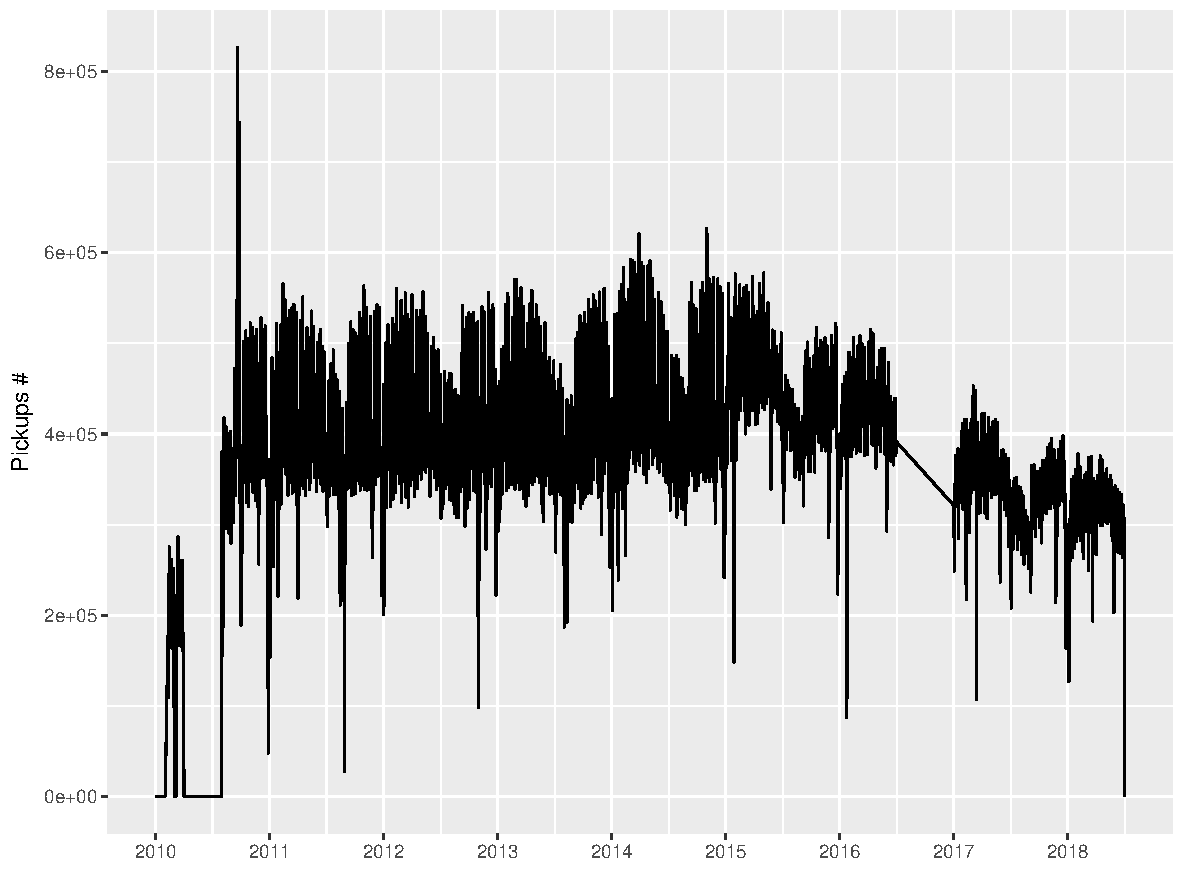
\includegraphics[width=1\columnwidth]{resources/base_plots/overall_pickups.pdf}
	\caption{Pickups count by day. Notice the decline in taxi pickups started in 2015.}
	\label{fig:overallPickups}
\end{figure}

The study continues with the analysis of pickups and dropoffs. \cref{fig:overallPickups} shows the number of pickups as a function of time. As already suggested by \cref{fig:travelsByYear} we notice a significant decrease in taxi service popularity starting from 2015. As depicted in \cref{fig:pickupHourDist} we can see that the periods of major activity for pickups are 8-16 and 20-24. The dropoffs follow the same pattern. Interestingly, by looking at the variation of the average speed through the day, as shown in \cref{fig:speedByHour}, we note that there is an inverse relationship between number of pickups and average speed, suggesting that in the highlighted time frames the city is subject to higher traffic congestions.
The most active pickup zones, as we can see from \cref{fig:pickupDistributionMap}, are Manhattan, the part of Brooklyn closer to Manhattan, LaGuardia and JFK airports. The dropoff zones closely follow the pattern of the pickup zones, but are slightly more evenly distributed across all zones. \cref{fig:pickupDropoffImageMap} highlights the situation, showing that dropoff locations are more granularly distributed with respect to pickup locations. It must be noted however that the majority of the activity is concentrates in the most profitable Manhattan and airport sectors.
We also note that, as illustrated in \cref{fig:speedMap}, the average speed per pickup location is inversely proportional to the number of pickups in that location, with the slowest zones being Manhattan, South Bronx and North Brooklyn. We can assume this zones to be the most subject to traffic.

\begin{figure}
	\centering
	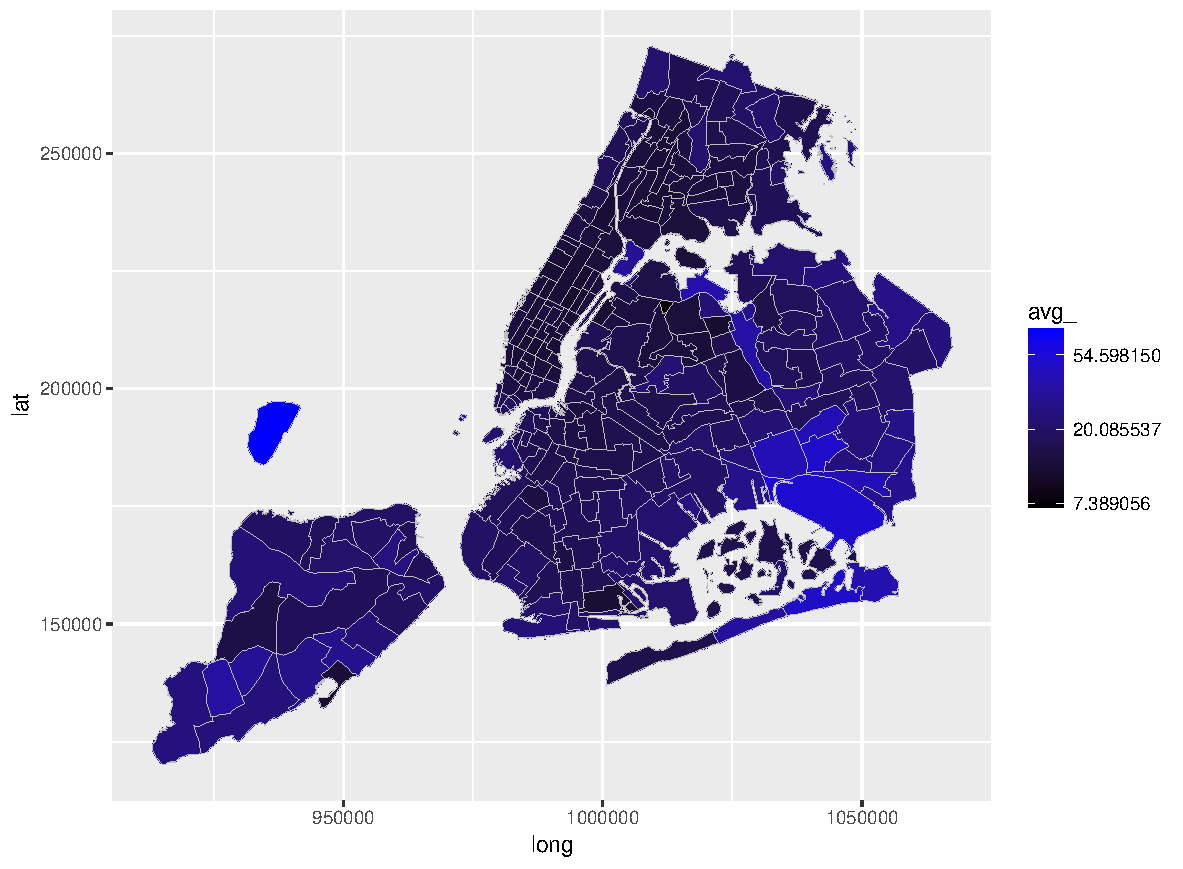
\includegraphics[width=1\columnwidth]{resources/base_plots/avg_total_amount_by_pickup_location_map.pdf}
	\caption{Map showing the average total amount by pickup location. Notice the inverse relationship with the distance from Manhattan.}
	\label{fig:totalAmountMap}
\end{figure}

\begin{figure}
	\centering
	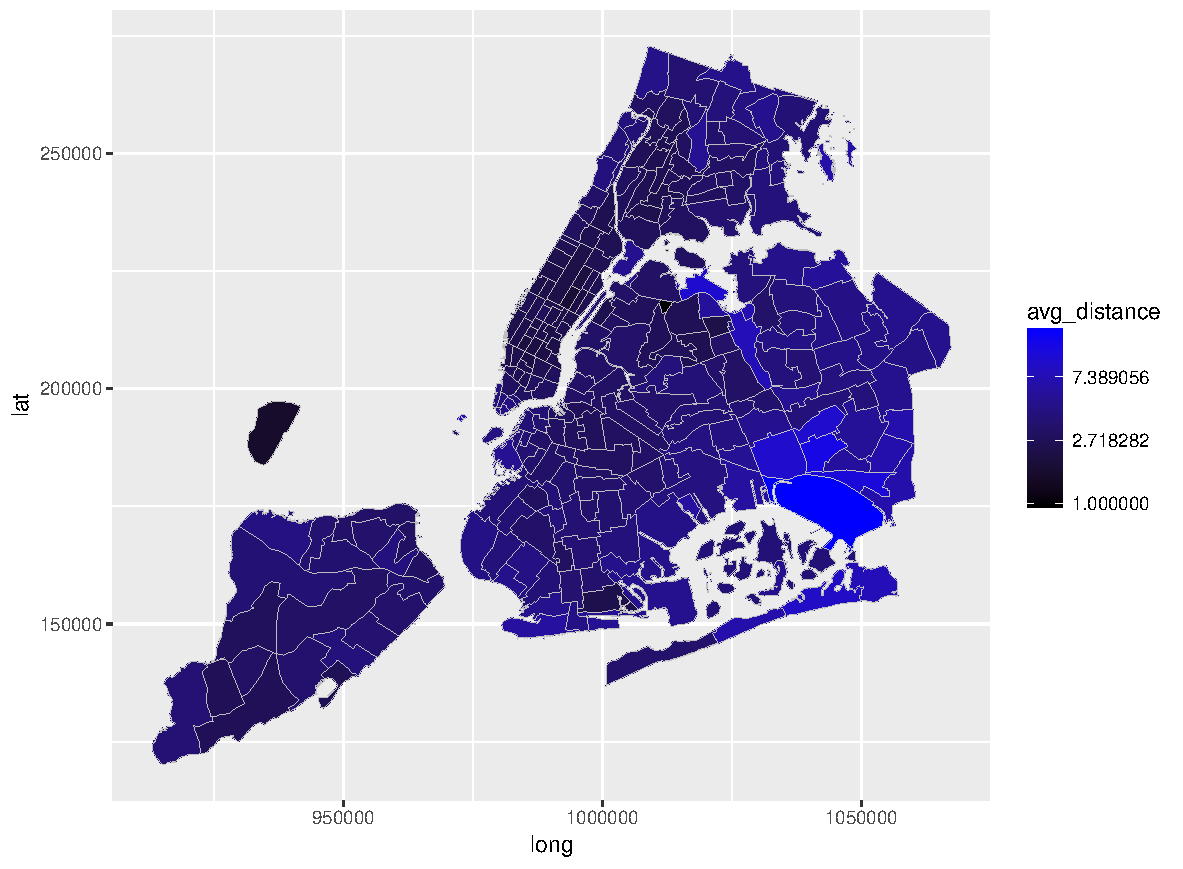
\includegraphics[width=1\columnwidth]{resources/base_plots/avg_distance_by_pickup_location_map.pdf}
	\caption{Map showing the number the average trip distance by pickup location. Notice the inverse relationship with the distance from Manhattan and the correlation with the average total amount map.}
	\label{fig:distanceMap}
\end{figure}

\begin{figure}
	\centering
	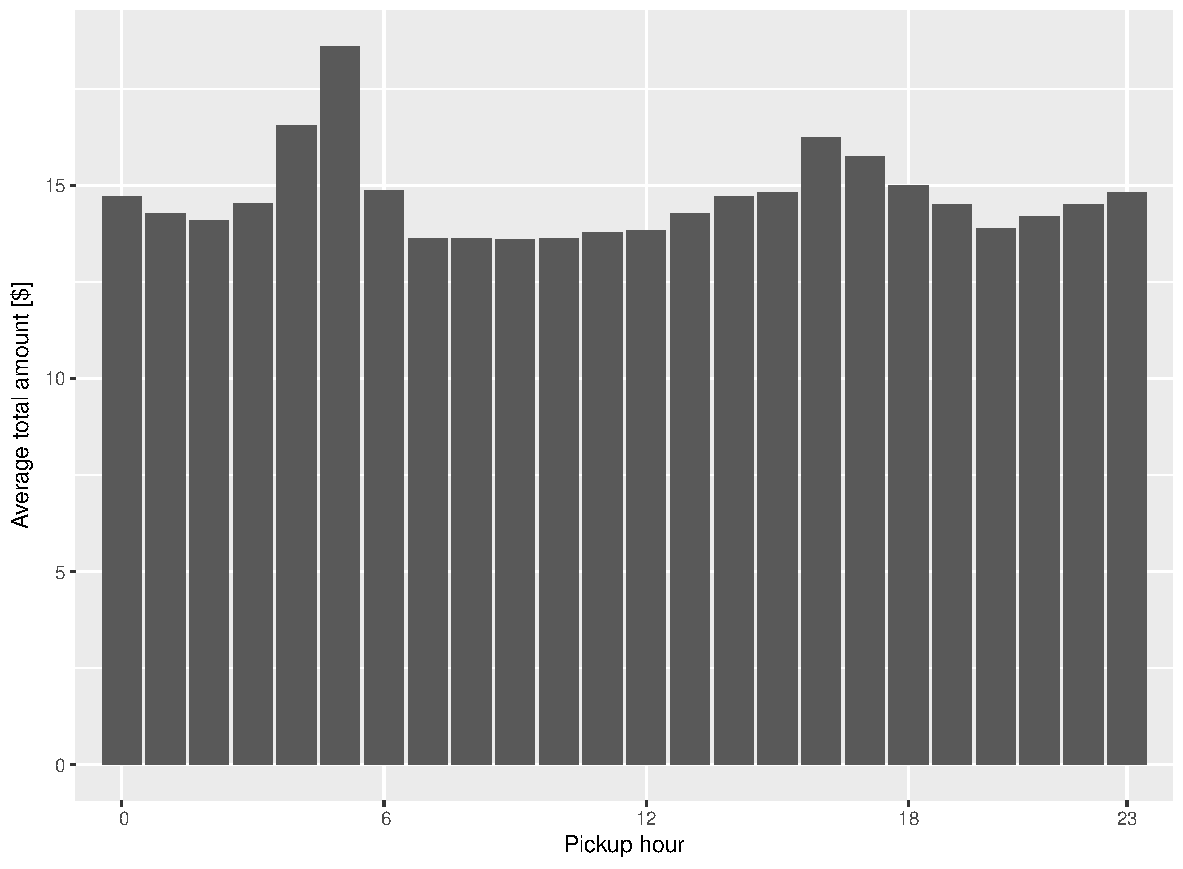
\includegraphics[width=1\columnwidth]{resources/base_plots/avg_total_amount_by_pickup_hour.pdf}
	\caption{Average total amount divided by pickup hour. Notice the two peaks at 5 and 16.}
	\label{fig:totalAmountByHour}
\end{figure}

\begin{figure}
	\centering
	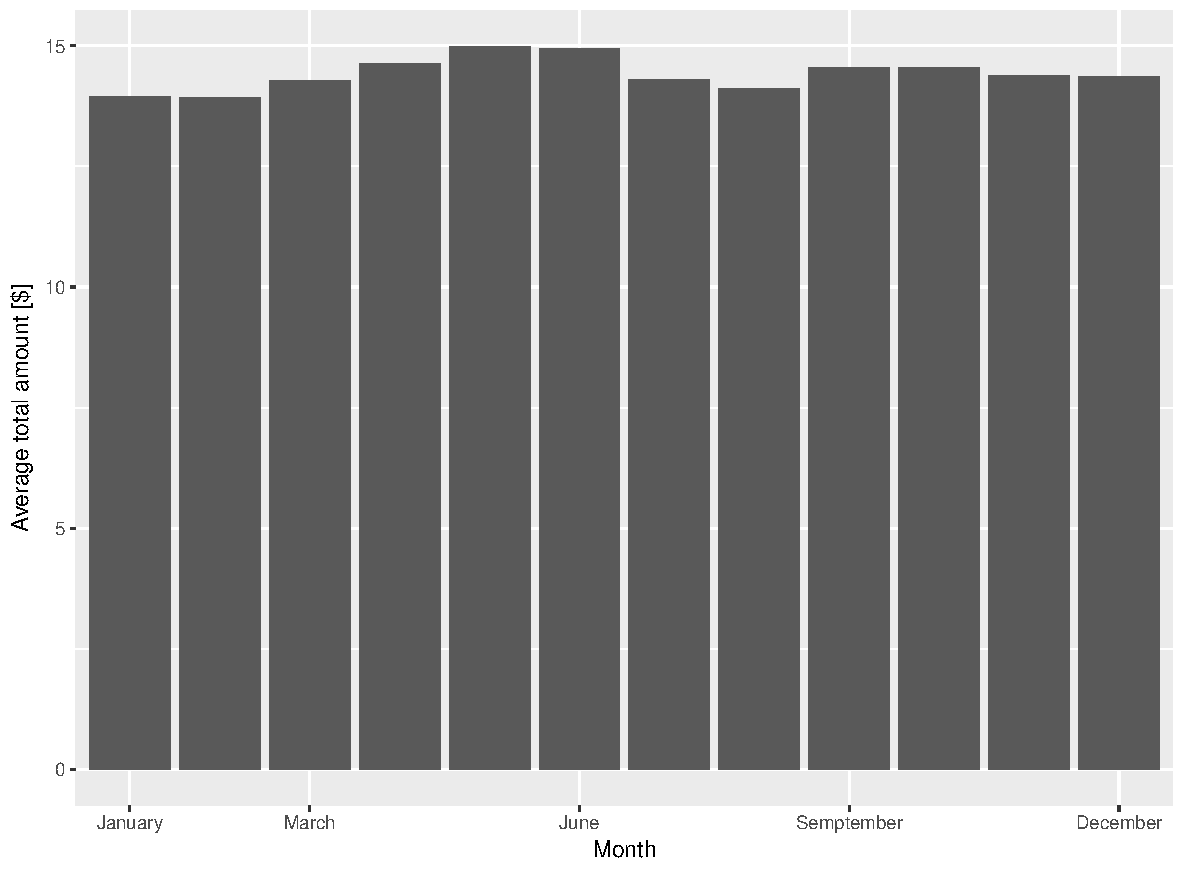
\includegraphics[width=1\columnwidth]{resources/base_plots/avg_total_amount_by_month.pdf}
	\caption{Average total amount divided by month. May and September-October result the most profitable periods.}
	\label{fig:totalAmountByMonth}
\end{figure}

It is also interesting to notice how total amounts relate to the pickup location. As depicted in \cref{fig:totalAmountMap} it can be noted that there is an inverse relationship between average total amount and zone distance from Manhattan. This is an expected outcome of the fact that Manhattan is one of the favourite dropoff locations, so on average the furthest zones from it are the most expensive. \cref{fig:distanceMap} shows the average trip distance by pickup location. Here we can note the direct correlation with the average total amount of the preceding picture. The average total amount also varies during the day, as depicted in \cref{fig:totalAmountByHour}. Two different peak periods are identified around 5 and 16. The discontinuity at 16 is caused by the introduction of a 1\$ extra from 16 to 20 as a standard component of the fare amount, while the peak at 5 is caused by a sharp increase in the average trip distance from 2.92 to 4.61 miles due to an increased proportion of people going to the airport early in the morning with respect to the normal traffic. It can also be noted from \cref{fig:totalAmountByMonth} that the average total amount varies during the months, with most profitable periods being May and September-October.

\begin{figure}
	\centering
	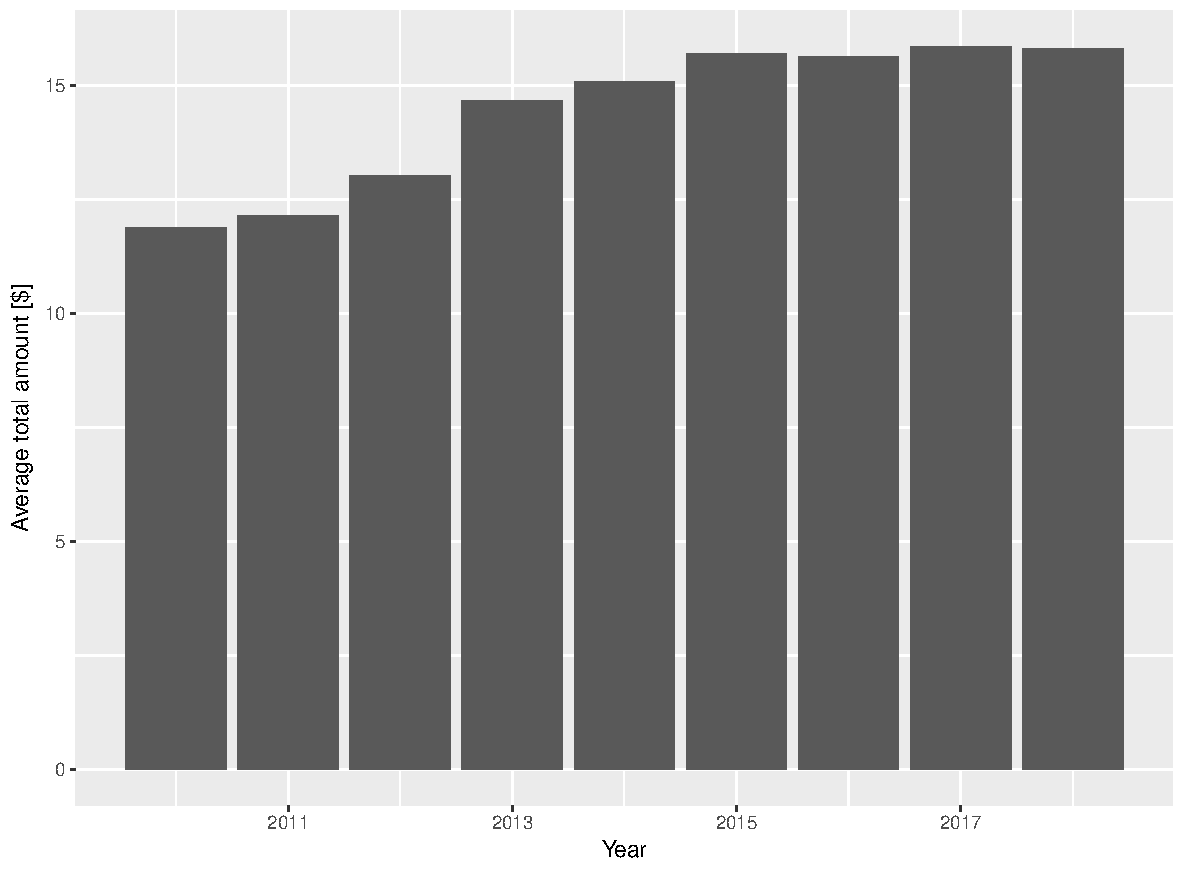
\includegraphics[width=1\columnwidth]{resources/base_plots/avg_total_amount_by_year.pdf}
	\caption{Average total amount by year. In 2012 the New York taxi commission increased the fare rates.}
	\label{fig:totalAmountByYear}
\end{figure}

\begin{figure}
	\centering
	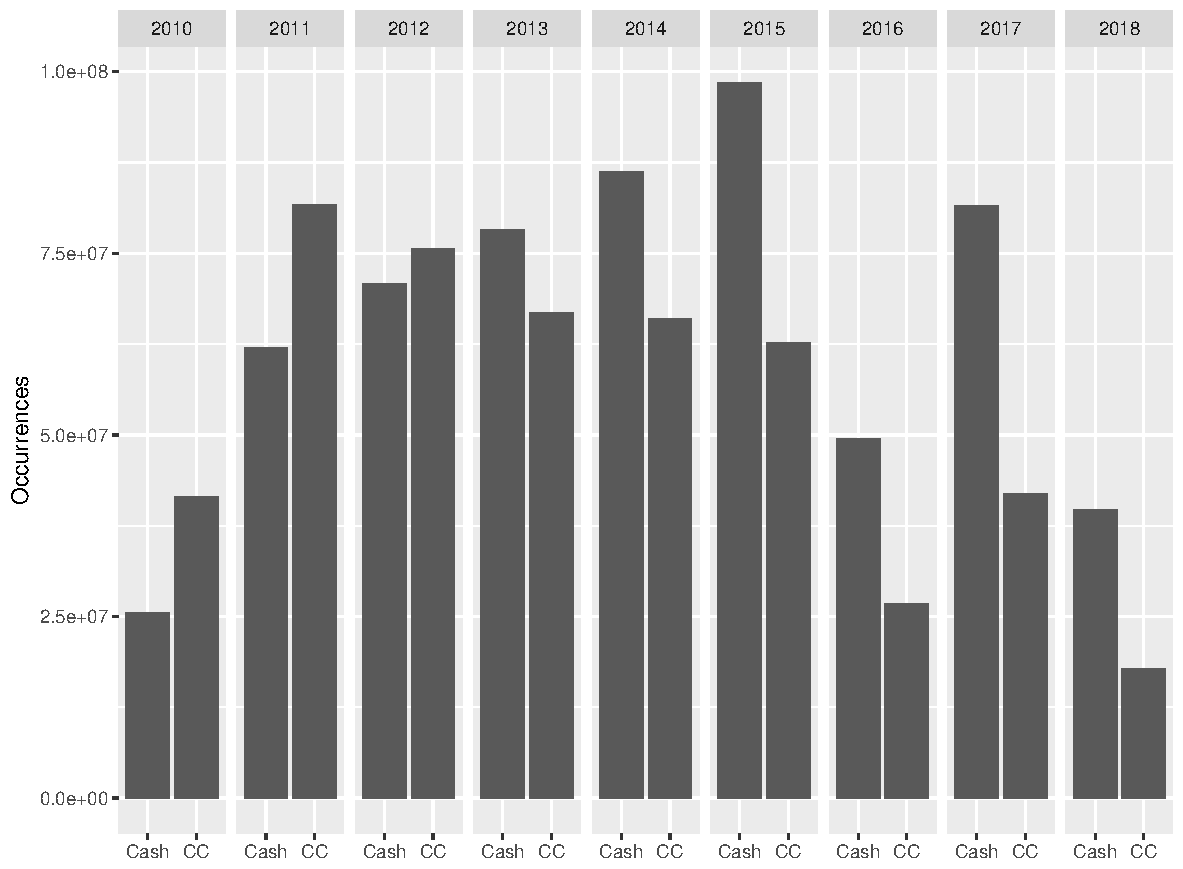
\includegraphics[width=1\columnwidth]{resources/base_plots/payment_type_distr.pdf}
	\caption{Distribution of payment types during the years. Notice the steady decline of cash payments in favor of credit card payments.}
	\label{fig:paymentTypeByYear}
\end{figure}

\begin{figure}
	\centering
	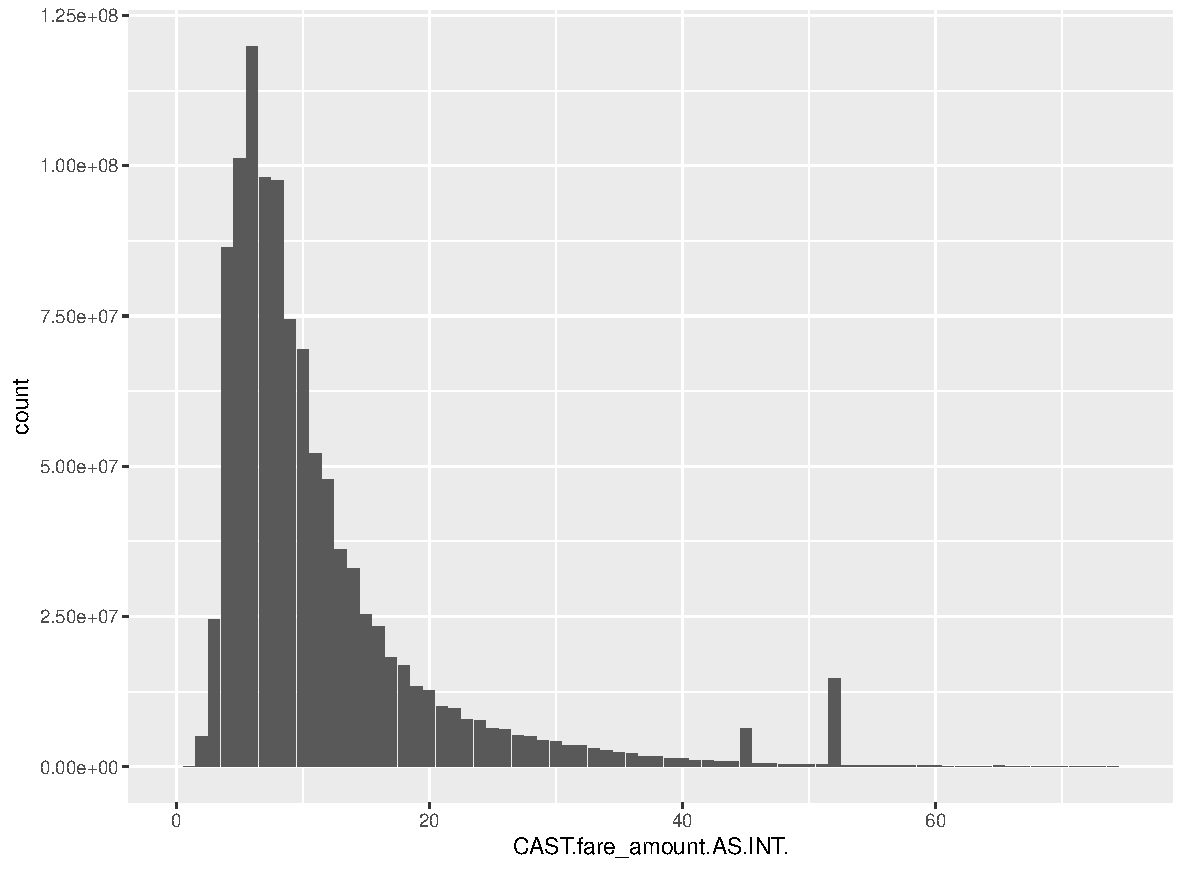
\includegraphics[width=1\columnwidth]{resources/base_plots/fare_amount_distr.pdf}
	\caption{Distribution of fare amounts. Notice the peaks at 45\$ and 52\$ corresponding to the JFK airport flat rates before and after the 2012 fares revision operated by the New York taxi commission.}
	\label{fig:fareAmountDistr}
\end{figure}

\begin{figure}
	\centering
	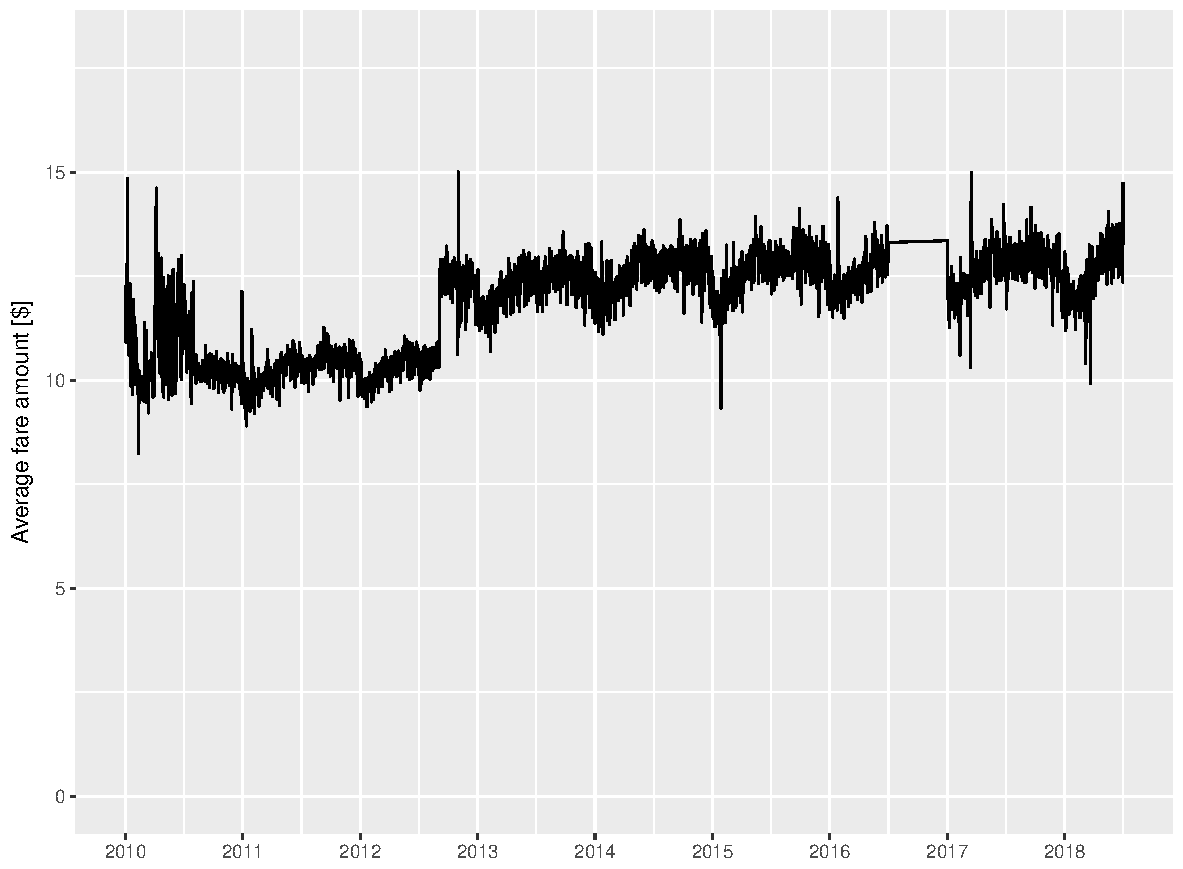
\includegraphics[width=1\columnwidth]{resources/base_plots/overall_fare_amount.pdf}
	\caption{Average fare amount by day in \$. Notice how in 2012 the new fare system caused a prominent increase in fare rates.}
	\label{fig:overallFareAmount}
\end{figure}

We also noted a general increase of the total amount during the years, as noted in \cref{fig:totalAmountByYear}, which is a consequence of many factors. First, the average fare amount passed from 10.18\$ of 2010 to 12.61\$ of 2018 due to a general revision of fare rates operated by the New York taxi commission in 2012 which can be seen in \cref{fig:overallFareAmount}. Other factors include slight increases in the average tolls, extras and improvement surcharge during the years. It must be noted however that the increase is exacerbated by the fact that total amounts in our datasets include tips only for trips paid with credit card and that during the years there has been a constant increase in the use of credit cards as shown in \cref{fig:paymentTypeByYear}. If our dataset included also cash tips, then we would still notice an increase in the total amount during the years, although more subtle.
The overall distribution of fare amounts is shown in \cref{fig:fareAmountDistr}. Note the sharp discontinuities at 52\$ and 45\$. These represents the special fare rate of trips linking Manhattan to the JFK airport, before and after a general revision of fare rates operated by the New York taxi commission during 2012.

A consistent part of the total amount is given by tips. A calculation of average tips percentages, calculated only on credit card paid trips, shows that the typical trip is tipped 18.6\% and this rate remains stable in all the analyzed years. This value corresponds to the guidelines of many online sources that suggest tipping taxi drivers from 15\% to 20\% of the total amount.

\begin{figure}
	\centering
	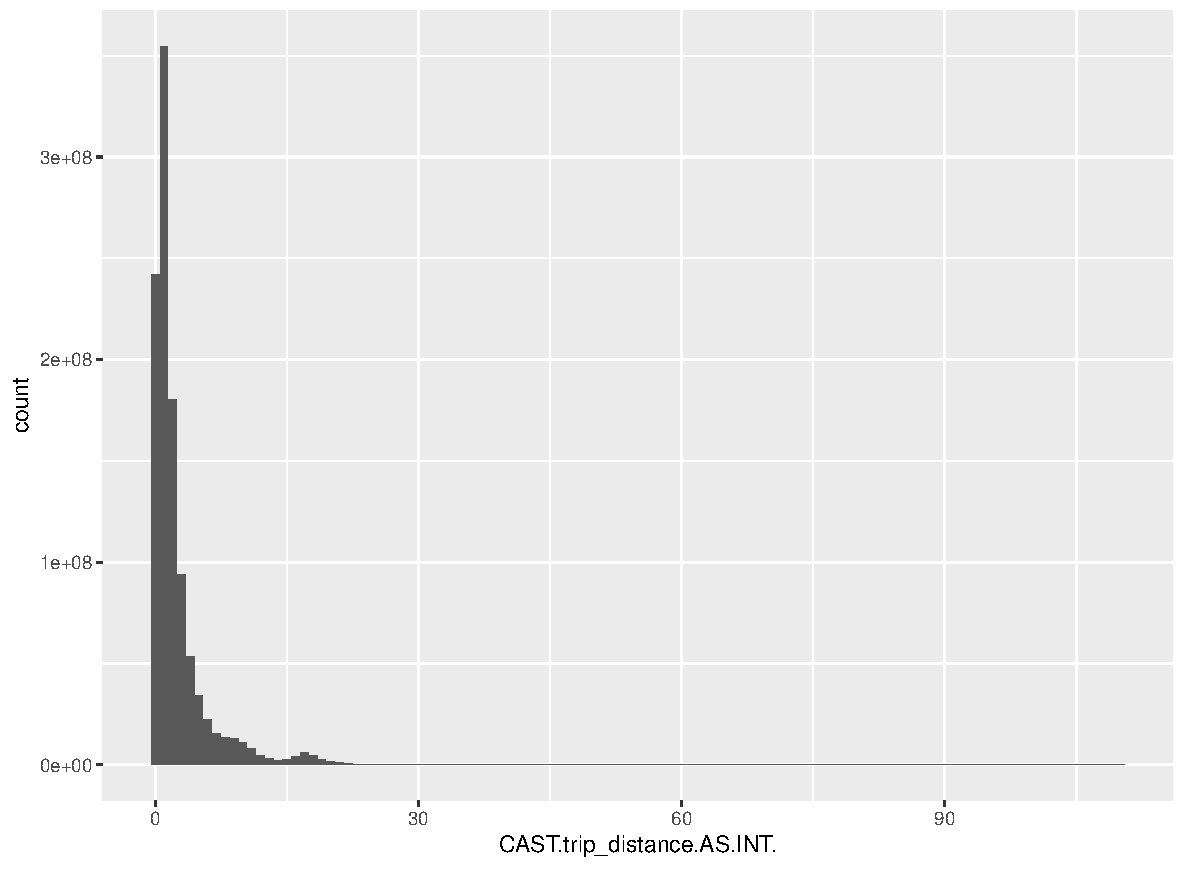
\includegraphics[width=1\columnwidth]{resources/base_plots/trip_distance_distr.pdf}
	\caption{Distribution of trip distances. Notice the three modes at 1, 9 and 17 miles.}
	\label{fig:tripDistanceDistr}
\end{figure}

Other interesting findings regard the distribution of trip distances which is shown in \cref{fig:tripDistanceDistr}. It can be observed that the distribution is trimodal, with the first mode at 1 mile, which represents short trips performed mainly inside Manhattan, the second at 9 miles, which represents trips between Manhattan and LaGuardia airport, and the third at 17 miles, which represents trips between Manhattan and JFK airport.

\begin{figure}
	\centering
	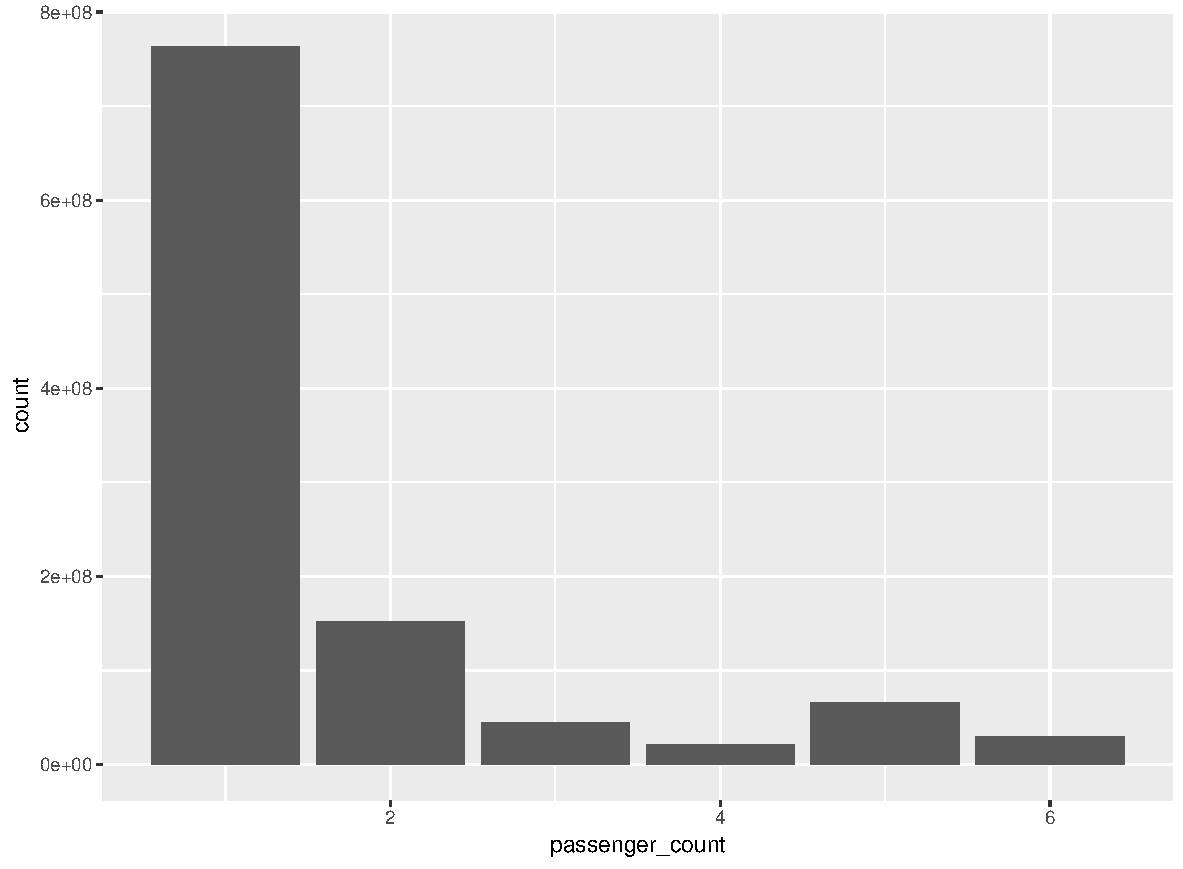
\includegraphics[width=1\columnwidth]{resources/base_plots/passenger_count_dist.pdf}
	\caption{Distribution of the number of passengers.}
	\label{fig:passengerCountDistr}
\end{figure}

Looking at the passenger count distribution in \cref{fig:passengerCountDistr} we can note that the majority of trips is performed with 1 or 2 passengers, while there is also a component of group rides which causes a peak at 5 passengers.

By looking at the distribution of payment types during the years in \cref{fig:paymentTypeByYear} it can be noted a strong trend towards paying with credit card versus cash, which was prevalent until 2012.

\begin{figure}
	\centering
	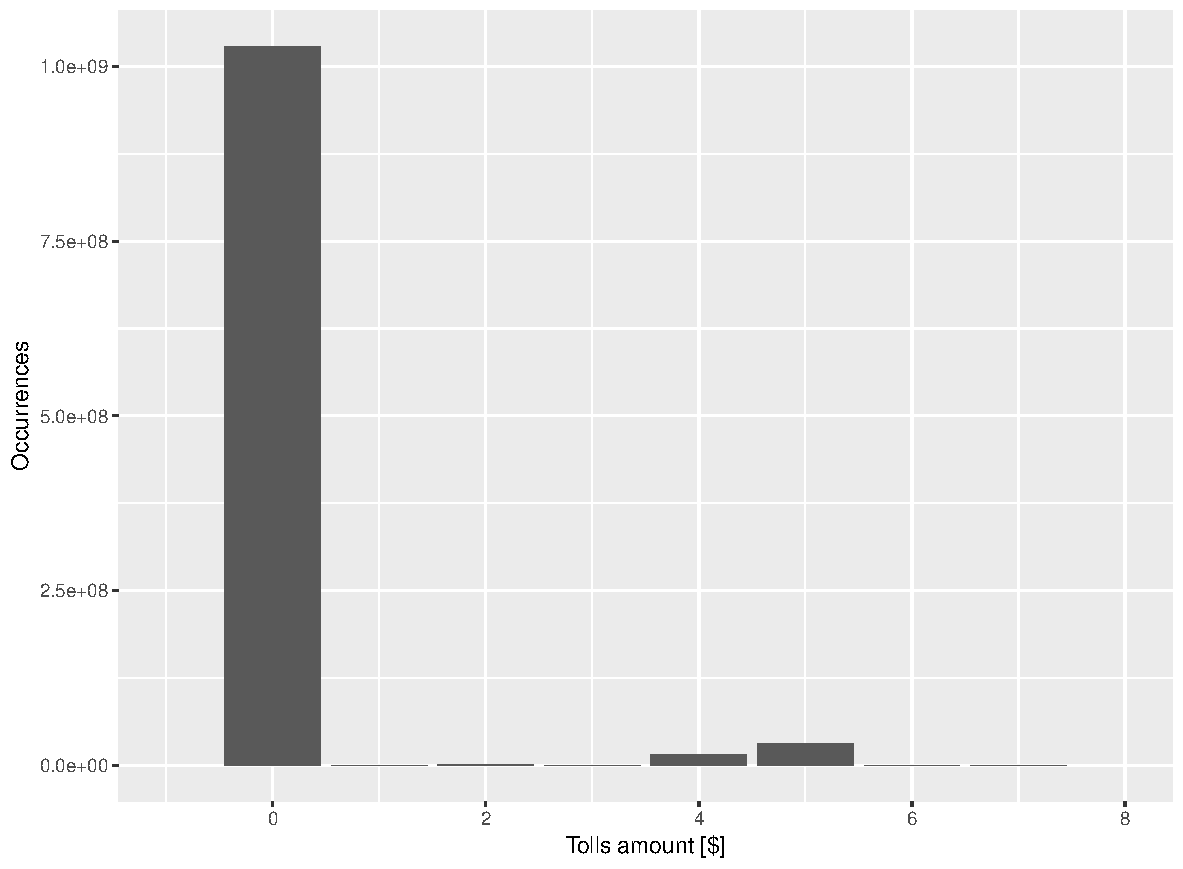
\includegraphics[width=1\columnwidth]{resources/base_plots/tolls_amount_distr.pdf}
	\caption{Distribution of tolls amount. Notice the modes at 0\$ and 5\$.}
	\label{fig:tollsAmountDistr}
\end{figure}

As a last general remark, we note that the distribution of tolls amount, as shown in \cref{fig:tollsAmountDistr}, is bimodal, with the first mode at 0\$ and a smaller mode at 5\$, representing the fact that the majority of trips are not subject to tolls, while the ones that are subject to them pay on average 5\$ of tolls. These correspond to tolls for Queens-Midtown Tunnel, Brooklyn-Battery Tunnel and the Triboro Bridge, which are convenient ways to avoid traffic for reaching the various parts of Manhattan from Brooklyn and Queens.

\section{Traffic segmentation}

After the data cleaning and preliminary analysis phase, we decide to perform a characterization of the different types of trips through k-means clustering. In order to perform an effective clustering, we introduce new features to the dataset and manipulate existing ones in order to guide the model towards finding interesting trends in the data. The following features are given to the clustering algorithm:

\begin{itemize}
	\item taxi company, boolean field representing whether the trip was served by yellow or green taxis
	\item pickup hour and dropoff hour, scaled integer fields representing the hour of pickup and dropoff
	\item weekend, boolean field set to true if the trip happened during the weekend
	\item passenger count, scaled numerical field representing the number of passengers
	\item speed, scaled numerical field representing average speed
	\item distance, scaled numerical field representing metered distance
	\item ratecode id, one hot encoded field representing the used ratecode
	\item fare amount, scaled numerical field representing metered fare
	\item tolls amount, scaled numerical field representing the incurred tolls
	\item payment type, one hot encoded field representing the payment method
\end{itemize}  

Note that, as our objective is to find a global characterization of trip types which possible span the entire city, we do not include pickup and dropoff zone ids as clustering features because this would cause the algorithm to divide trips based on their starting or ending point which does not carry useful information. Notice also that we scaled every numerical field by its mean and variance. Without doing so, features with a wide range such as the fare amount would be the only ones relevant for the algorithm, which is not the result we want to obtain.

\begin{figure}
	\centering
	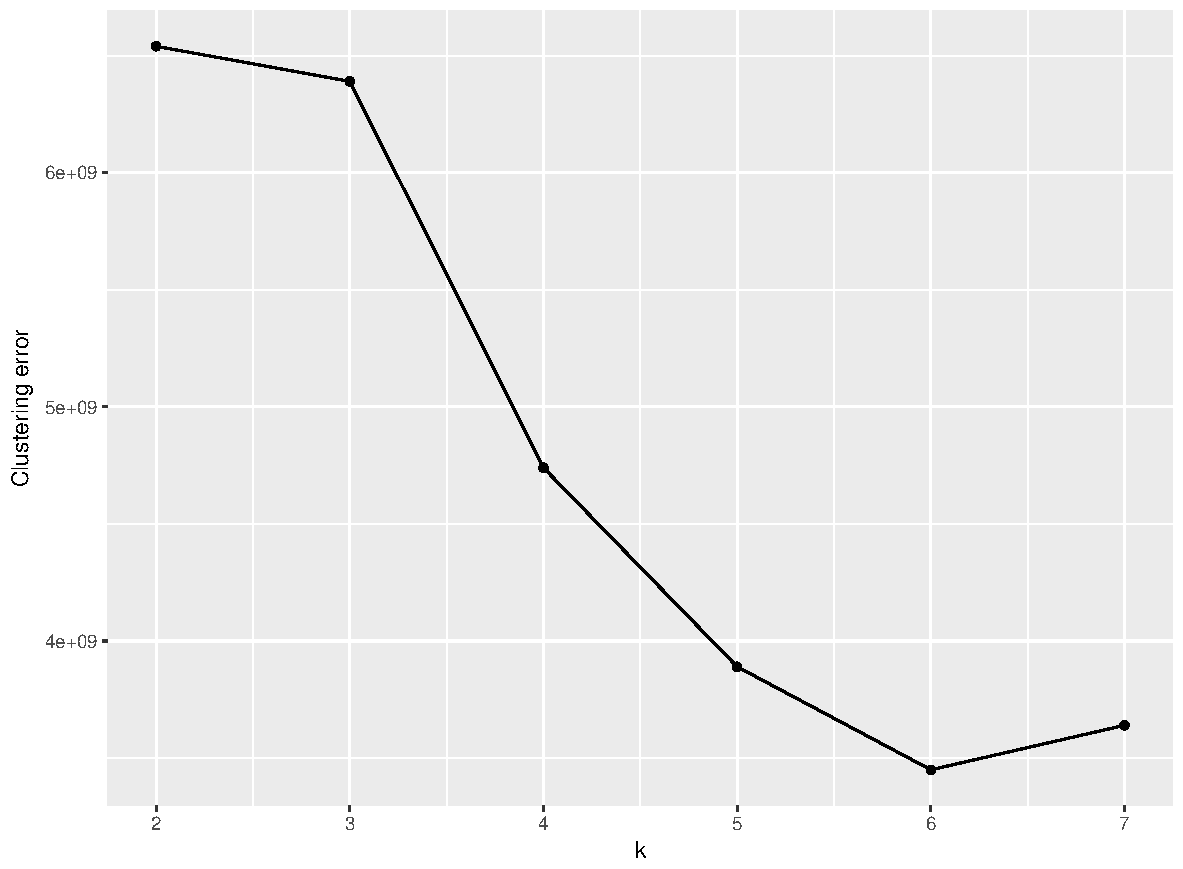
\includegraphics[width=1\columnwidth]{resources/clustered_plots/elbow.pdf}
	\caption{Representation of clustering error as a function of the number of clusters k. For performance reasons the error is estimated on a subportion of the dataset, so some points have an anomalous behavior. For k=5 we note that the error curve starts flattening, so 5 is chosen as the optimal k value.}
	\label{fig:elbow}
\end{figure}

\begin{figure}
	\centering
	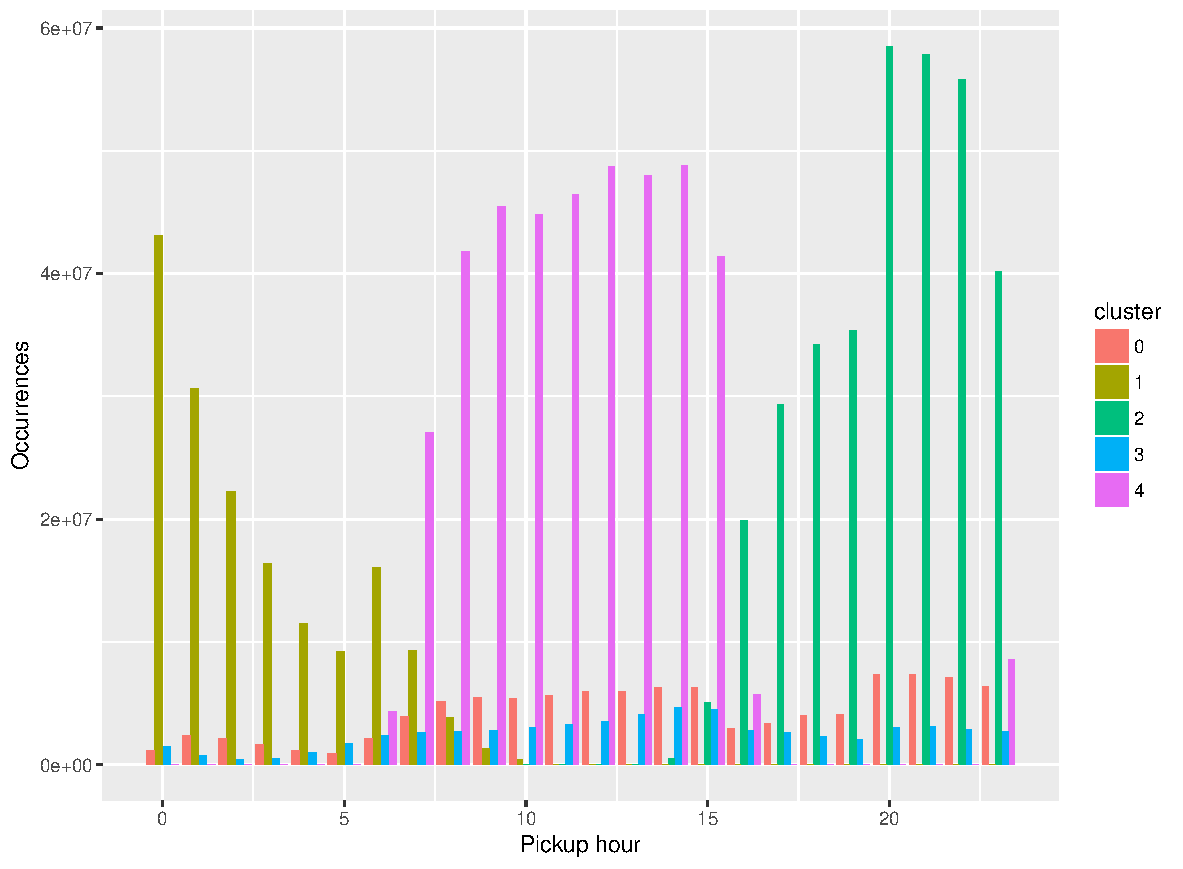
\includegraphics[width=1\columnwidth]{resources/clustered_plots/pickup_hour_dist.pdf}
	\caption{Number of pickups by day hour and cluster. Notice how clusters 1, 4 and 2 are determined based on the pickup hour.}
	\label{fig:clusterPickupHour}
\end{figure}
\begin{figure}
	\centering
	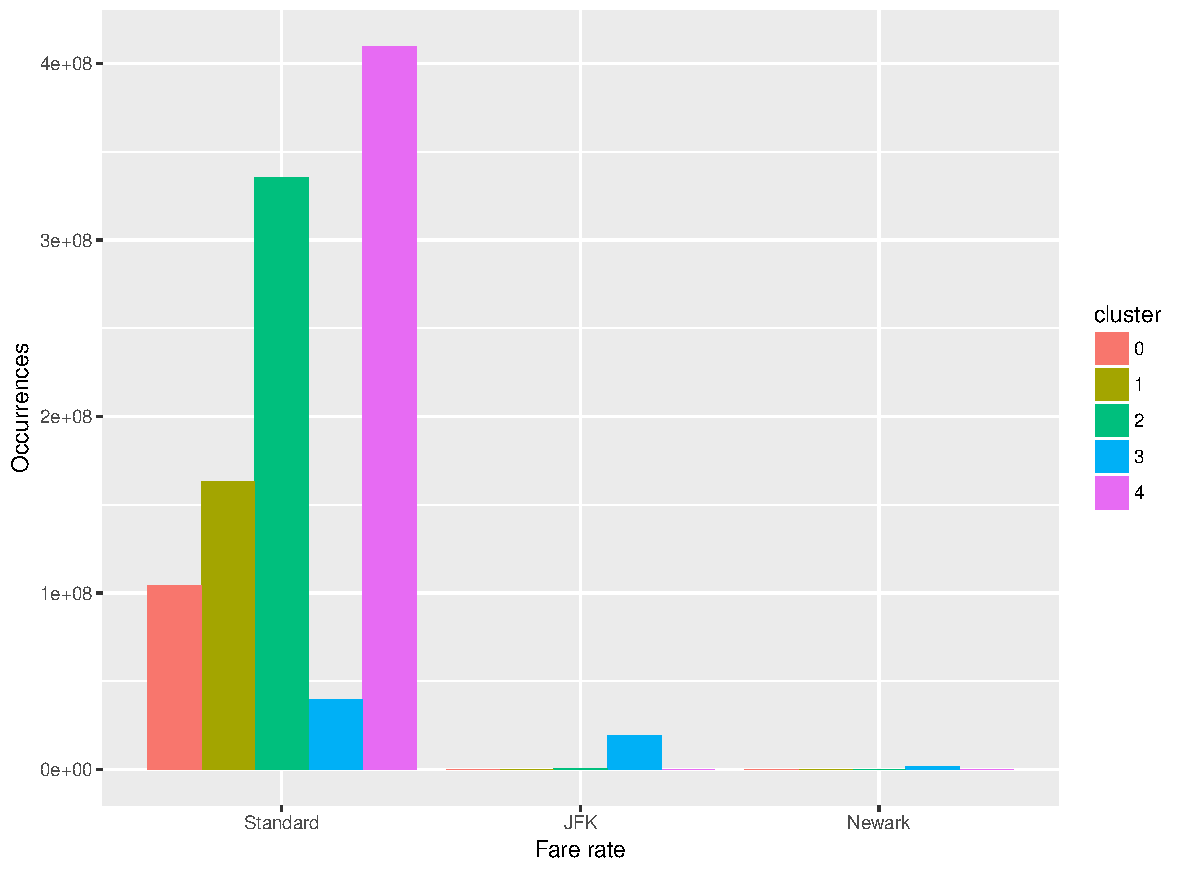
\includegraphics[width=1\columnwidth]{resources/clustered_plots/ratecode_distr.pdf}
	\caption{Distribution ratecodes divided by cluster. Notice how the majority of JFK trips are grouped in cluster 3.}
	\label{fig:clusterRatecode}
\end{figure}
\begin{figure}
	\centering
	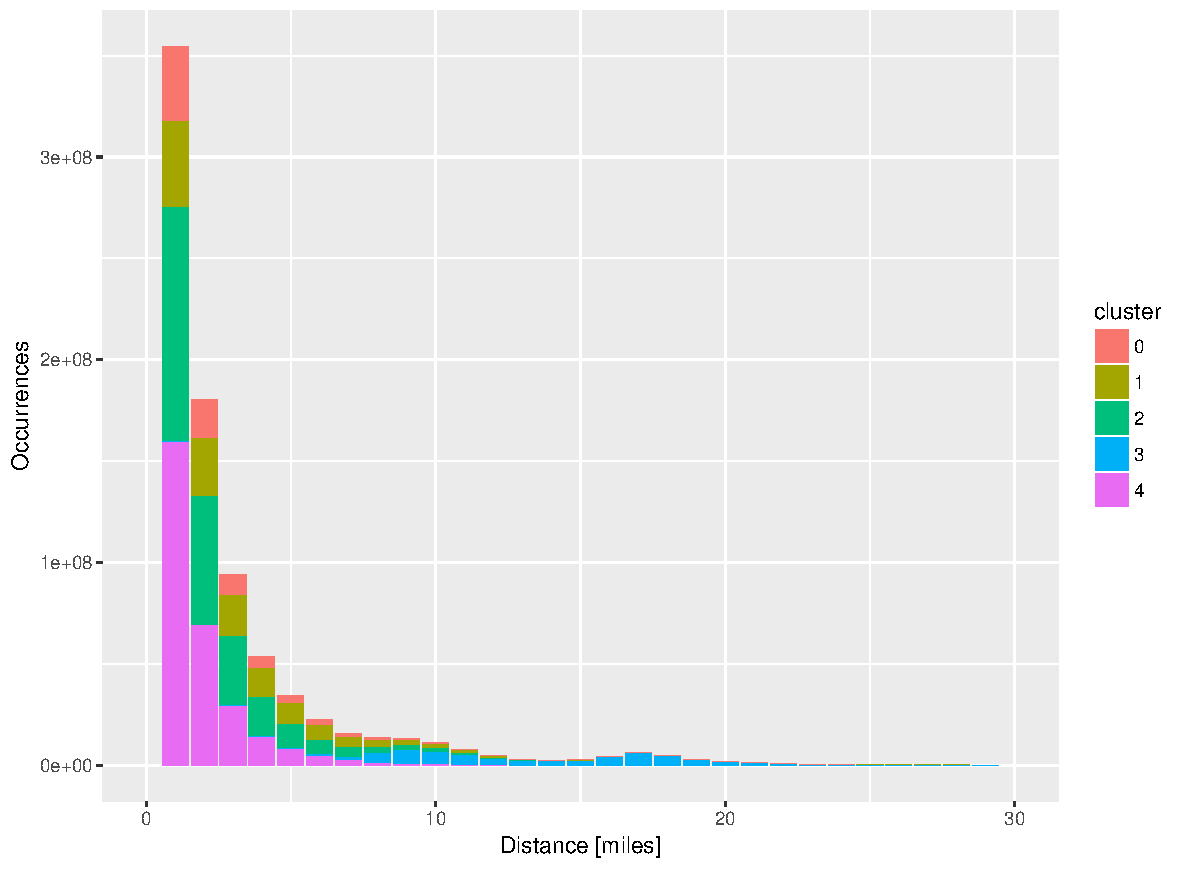
\includegraphics[width=1\columnwidth]{resources/clustered_plots/trip_distance_distr.pdf}
	\caption{Distribution of trip distance divided by cluster. Notice the modes for cluster 3 at 9 and 17 miles which corresponds respectively to trips to LaGuardia and JFK airport.}
	\label{fig:clusterDistance}
\end{figure}
\begin{figure}
	\centering
	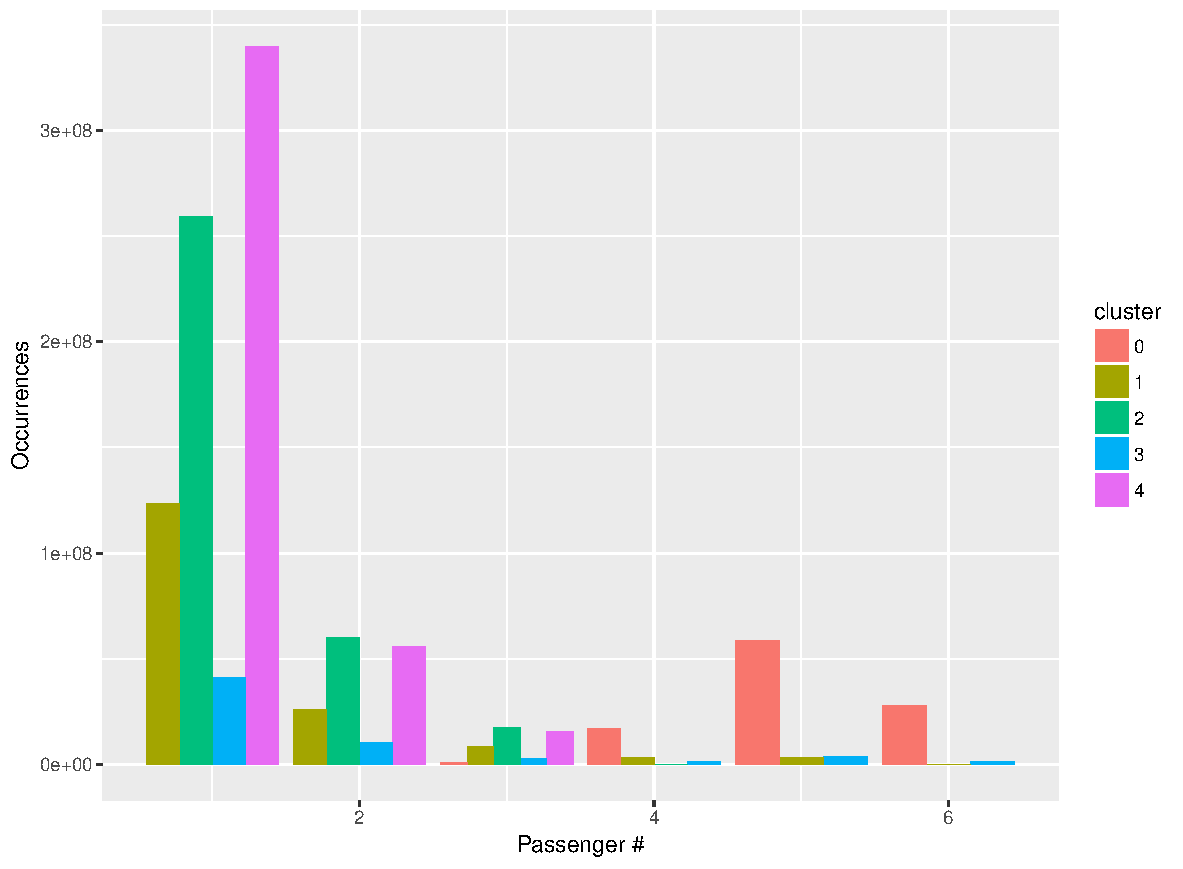
\includegraphics[width=1\columnwidth]{resources/clustered_plots/passenger_count_distr.pdf}
	\caption{Distribution of number of passengers per cluster.}
	\label{fig:clusterPassengerDistr}
\end{figure}

\begin{figure}
	\centering
	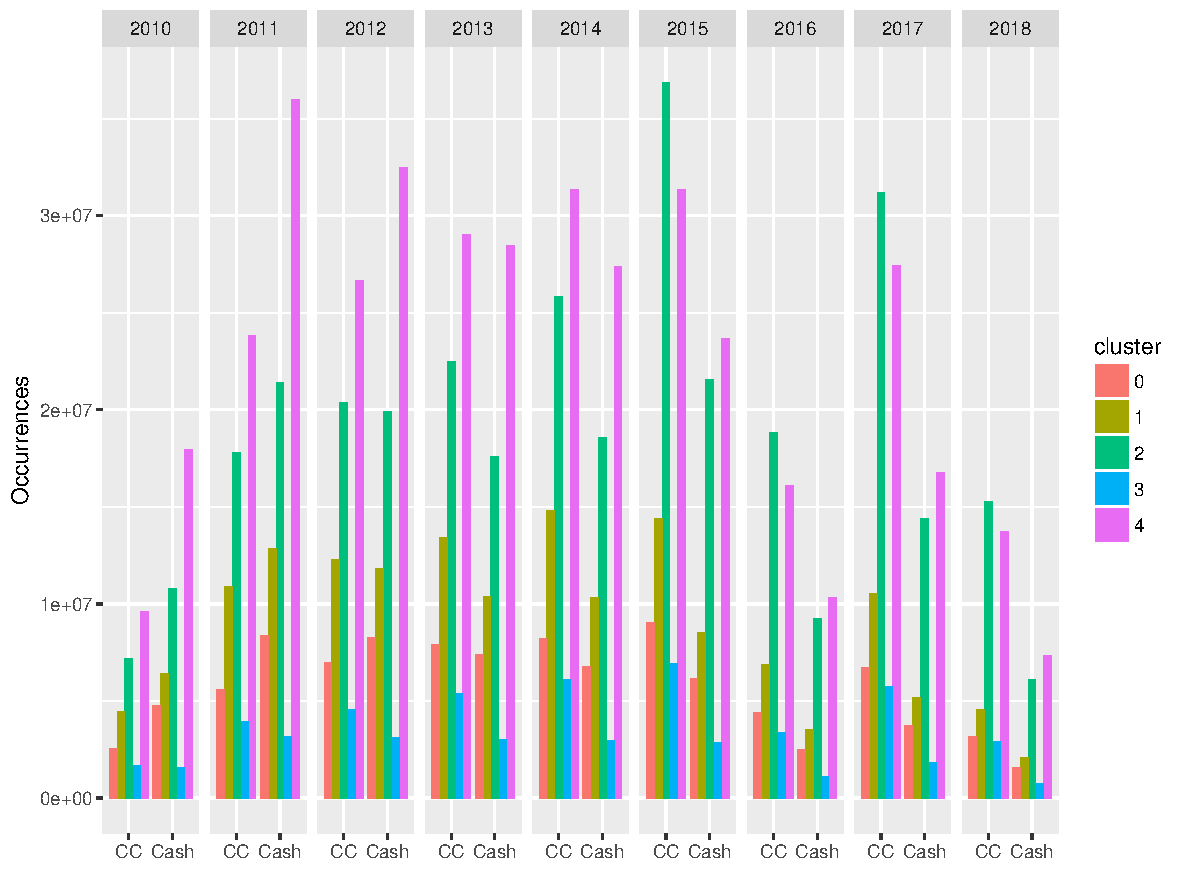
\includegraphics[width=1\columnwidth]{resources/clustered_plots/payment_type_distr.pdf}
	\caption{Distribution of payment types in time per cluster.}
	\label{fig:clusterPaymentType}
\end{figure}

\begin{figure}
	\centering
	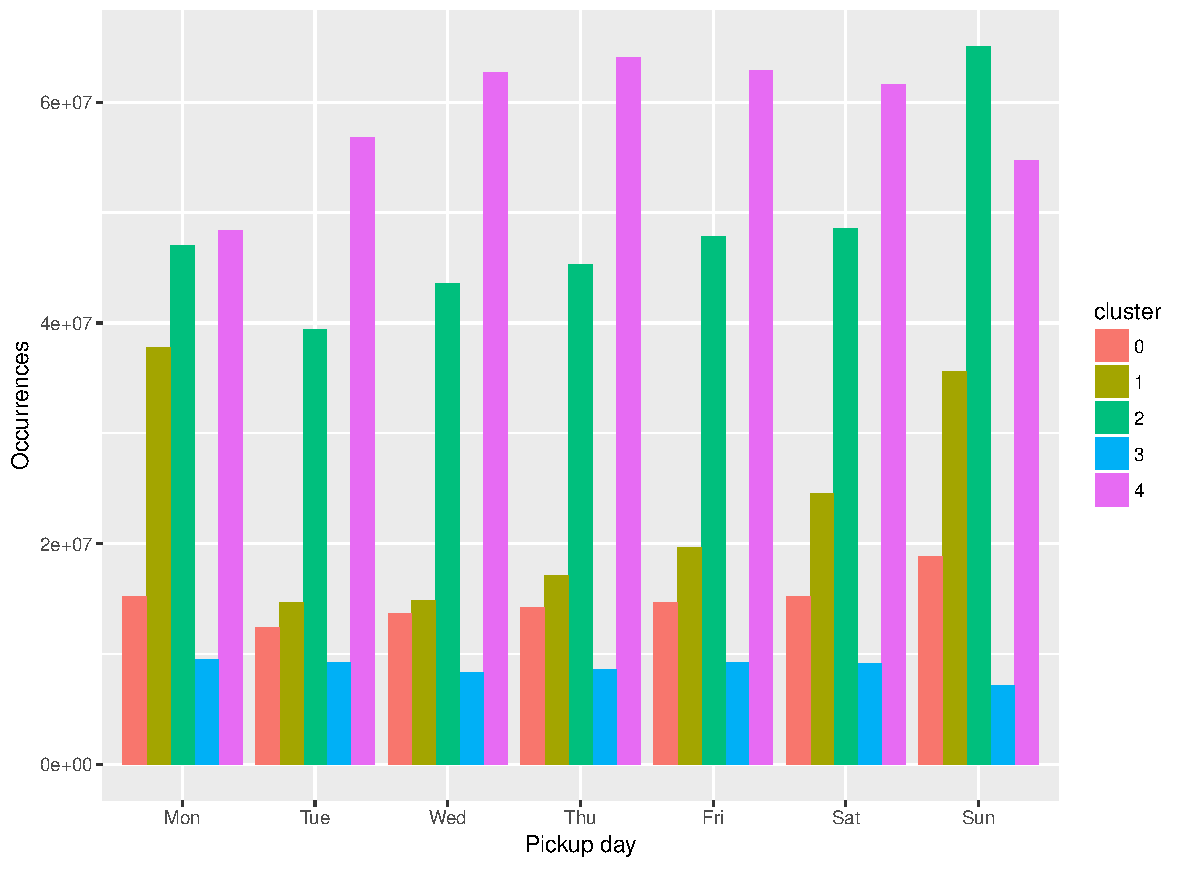
\includegraphics[width=1\columnwidth]{resources/clustered_plots/pickup_weekday_dist.pdf}
	\caption{Distribution across the week of the number of pickups per cluster.}
	\label{fig:clusterPickupDay}
\end{figure}


The appropriate number of clusters for the k-means clustering algorithm is detected using the Elbow method, which results are shown in \cref{fig:elbow}. For our dataset, the procedure suggested a number of cluster equal to 5. 

We then proceed to identify the characteristics of each of these 5 identified clusters. By looking at \cref{fig:clusterPickupHour}, we notice that cluster 1 corresponds to early morning trips done from 0 until 7, cluster 4 corresponds to day trip from 8 to 15 and cluster 2 corresponds to trip from 16 to 24. Furthermore, from \cref{fig:clusterRatecode} it can be seen that cluster 3 comprehends trips to JFK and Newark airports. Moreover, by looking at \cref{fig:clusterDistance} and by plotting the pickup locations on a map as a function of the cluster, we can also say that cluster 3 comprehends trips to LaGuardia airport. Lastly, by looking at \cref{fig:clusterPassengerDistr} we can see that cluster 0 corresponds to trips performed by groups of 4 or more people. We note also that cluster 1 and 2, that represent respectively early morning and night trips, could be unified in a single cluster with common characteristics. The reason why our clustering algorithm separated them is that the pickup and dropoff hour property cause trips in the evening to have a high distance measure from trips in the morning, while a more reasonable distance metric would use a circular similarity measure and assign to trips in the evening and trip in the morning a smaller distance.

By looking further into the data, we can notice from \cref{fig:clusterDistance} that day trips in cluster 2 tend to have a light tail, compared to heavy tails of clusters for morning and night trips and for group rides. This difference is probably explained by the fact that people tend to use taxis also for long and expensive trips at nights where the availability of other means of transport is reduced. From \cref{fig:clusterPaymentType} it can be noted that group rides and day trips tend to have a lower CC to Cash payment ratios, while airport trips, morning trips and night trips tent to be paid with credit card more frequently. It is also interesting to notice how these type of traffics vary through the week as shown in \cref{fig:clusterPickupDay}. Day trips tend to have their peak on Thursday and have lower activity along the weekend. On the other hand, group rides, morning trips and evening trips tend to peak in the weekend, probably because of the increased nightlife. Airport trips, on the other hand, have their peak on Monday and register their lowest point on Sunday.


\cref{fig:TrafficGraph} shows the graph constructed to better visualize the different types of traffic inside the city of New York. The number of edges, starting from a node, is variable and depends on the amount of pickups for that zone, this provides an immediate view of the most heavily trafficked areas of New York. Each node has a set of attributes describing: the level of activity, the average distance, duration, speed and total amount associated with the trips departing from that zone. Each of these attributes has a value between LOW, MEDIUM and HIGH calculated by finding the first and third quartiles of the corresponding distribution. The value of a given attribute for a node is considered LOW if it lies below the 25\% of the data in the dataset, MEDIUM if it lies between the 25\% and the 75\%, and HIGH for values above 75\%. An important aspect to note is that, in order to obtain a more comprehensible graph, the edges from a node to itself are removed.
From this graph it can observed that the majority of the trips tend to remain inside the same borough, also it can be seen that Manhattan is the borough with the highest traffic density, especially during the working hours. Inside this area some other interesting aspects can be noted. First, the zone of East Village is subject to a high amount of traffic especially in the evening, in fact this area is renowned for the nightlife. Second, the Roosevelt Island is not directly connected to any other zone in the same borough and this is confirmed by looking at its geographic location: it can be seen that, even though it is inside of the Manhattan borough, there is no direct path to Manhattan itself, and the only way to leave the island is through the Roosevelt Island Bridge which leads to Astoria in the Queens.
While looking at the Bronx borough, a less interconnected graph, representing a lower volume of activity, can be observed. It can be noticed that night trips are less frequent, this may be due to the level of criminality that discourages people from moving during these hours. 
Finally, the graph highlights that the clustering correctly identifies long distance trips, the majority of which is traffic towards the airports.
For the interactive version of the graph and its legend, please refer to \cref{sec:shared_folder}.

\begin{figure}
	\centering
	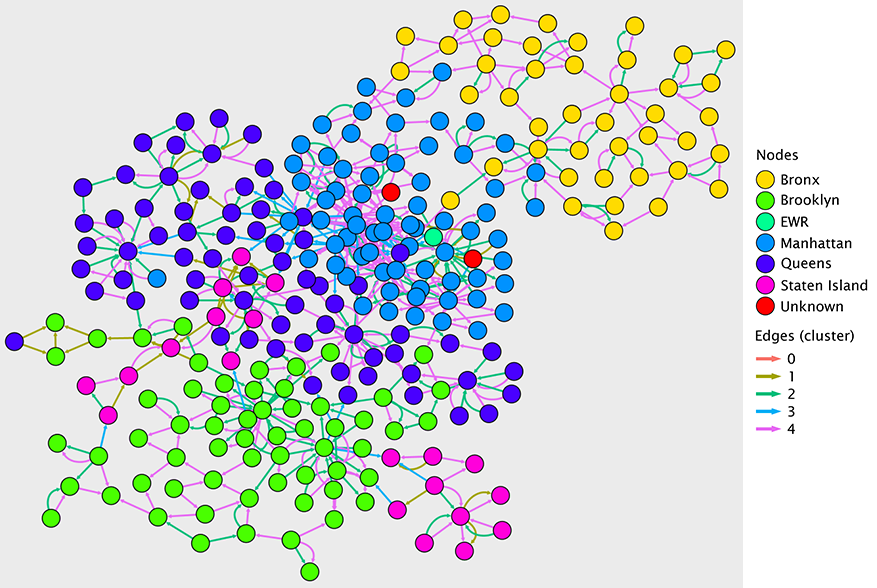
\includegraphics[width=1\columnwidth]{resources/traffic_graph.png}
	\caption{Directed graph showing the different types of traffic found using k-means clustering. Each node represents one of the 265 zones of New York, while each edge, between two zones, represents a traffic flow in the direction of the arrow. The colour of the nodes depends on the borough of the zone they represent. The colour of the edges depends on the type of traffic. For the interactive version of the graph and its legend see \cref{sec:shared_folder}}
	\label{fig:TrafficGraph}
\end{figure}

\section{Traffic flow analysis}

One of the objectives of this report is to better understand how people move inside the city of New York. We partially describe this activity in \cref{sec:preliminaryAnalysis} by showing the high activity levels of Manhattan and of the airport zones. In order to better understand the flows of traffic, we decide to plot, for each pickup borough, the distribution of dropoff locations as a function of time.

\begin{figure}
	\centering
	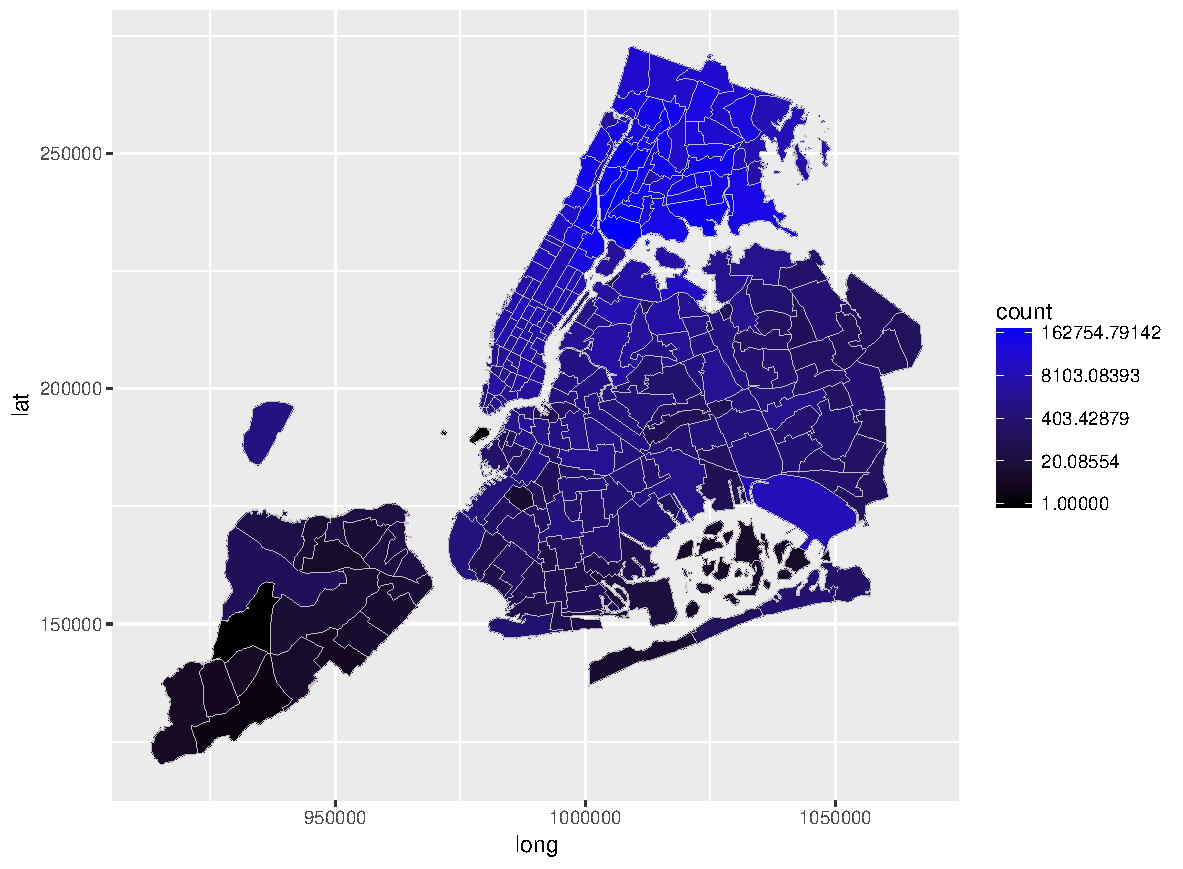
\includegraphics[width=1\columnwidth]{resources/base_plots/bronx_dropoff_location_id_dist_map.pdf}
	\caption{Map in logarithmic scale showing the preferred dropoff locations for rides starting inside the Bronx borough.}
	\label{fig:bronxDropoffMap}
\end{figure}

\cref{fig:bronxDropoffMap} shows the distribution of dropoff locations for pickups happened in the Bronx borough. The majority of dropoffs as expected happen inside the Bronx borough itself, North Manhattan or the two airports.

\begin{figure}
	\centering
	\subfloat[Overall dropoff locations (log scale)]{\label{fig:brooklynDropoffMap}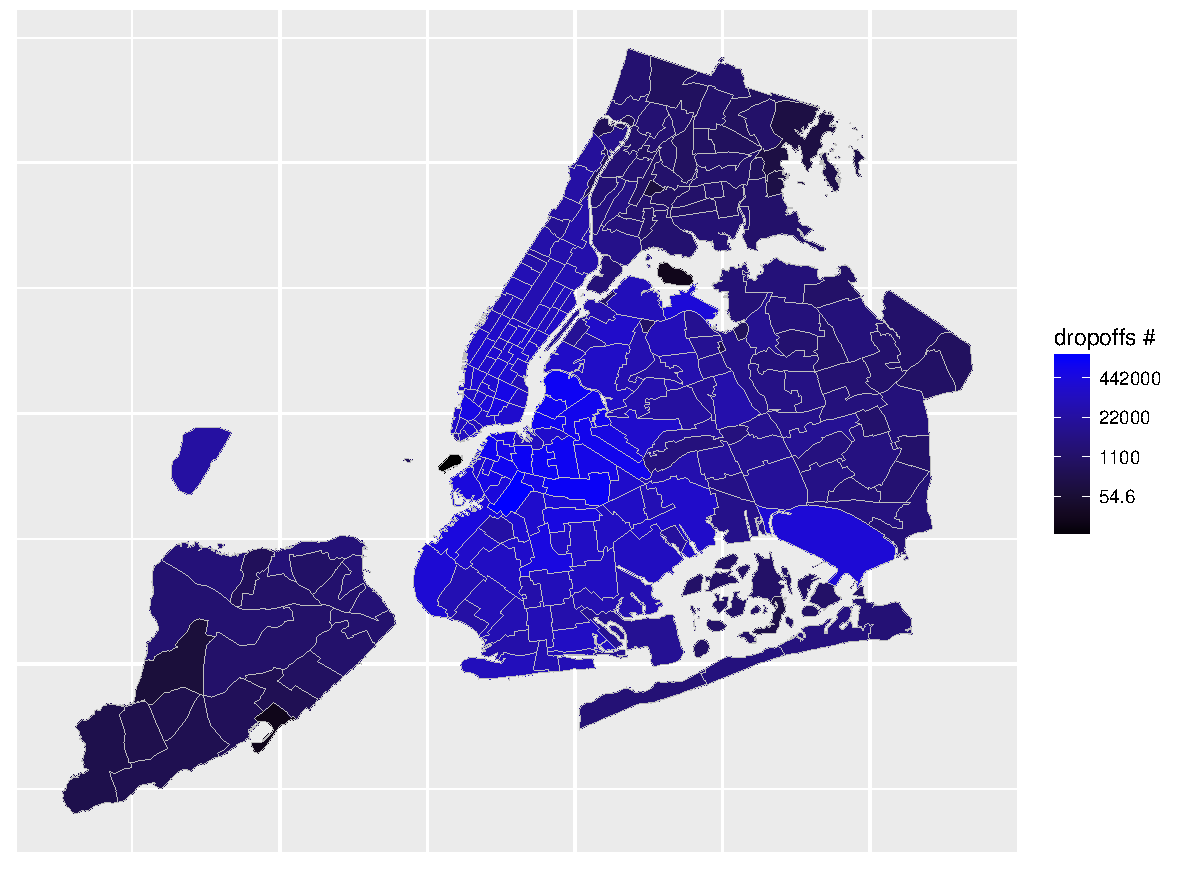
\includegraphics[width=1\columnwidth]{resources/base_plots/brooklyn_dropoff_location_id_dist_map.pdf}}\\
	\subfloat[Dropoff locations at 9]{\label{fig:brooklyn9DropoffMap}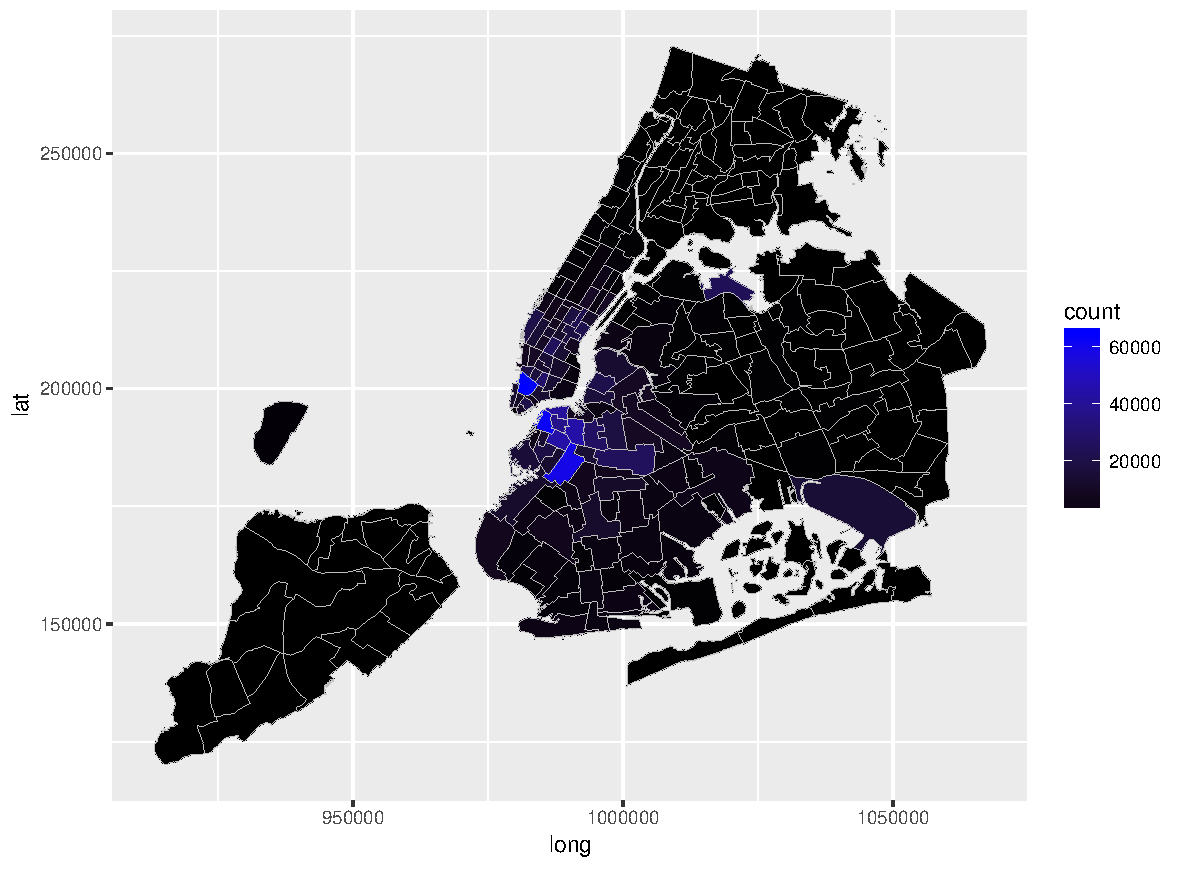
\includegraphics[width=1\columnwidth]{resources/base_plots/brooklyn_dropoff_location_id_by_pickup_hour_dist9_map.pdf}
	}
	\caption{Map showing the preferred dropoff locations for rides starting inside the Brooklyn borough, overall and at 9. Notice the high concentration of dropoffs in the Tribeca Manhattan district at 9.}
\end{figure}


\cref{fig:brooklynDropoffMap} highlights the distribution of dropoff locations for pickups happened in the Brooklyn borough. Also in this case, the majority of dropoffs happen inside the borough itself, the two airports or the adjacent Manhattan zones. An interesting consideration can be done by looking at \cref{fig:brooklyn9DropoffMap} which shows the favourite dropoff locations for rides beginning at 9. From 7 to 9 we can see a high rate of dropoffs in the Tribeca district of Manhattan, which is the ending point of the Brooklyn Bridge. This flow vanishes during the day and is probably caused by workers moving into the city early in the morning. 

\begin{figure}
	\centering
	\subfloat[Overall dropoff locations (log scale)]{\label{fig:manhattanDropoffMap}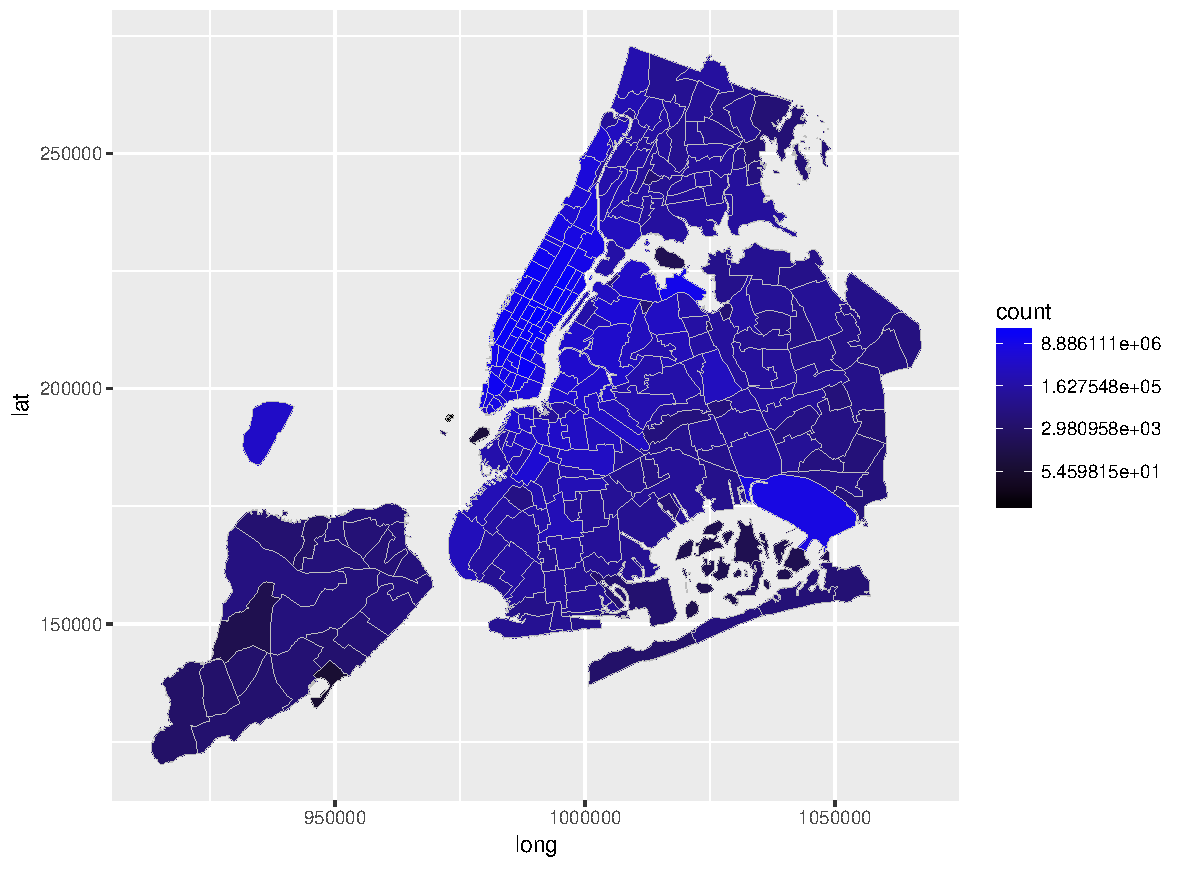
\includegraphics[width=1\columnwidth]{resources/base_plots/manhattan_dropoff_location_id_dist_map.pdf}}\\
	\subfloat[Dropoff locations at 10]{\label{fig:manhattan10DropoffMap}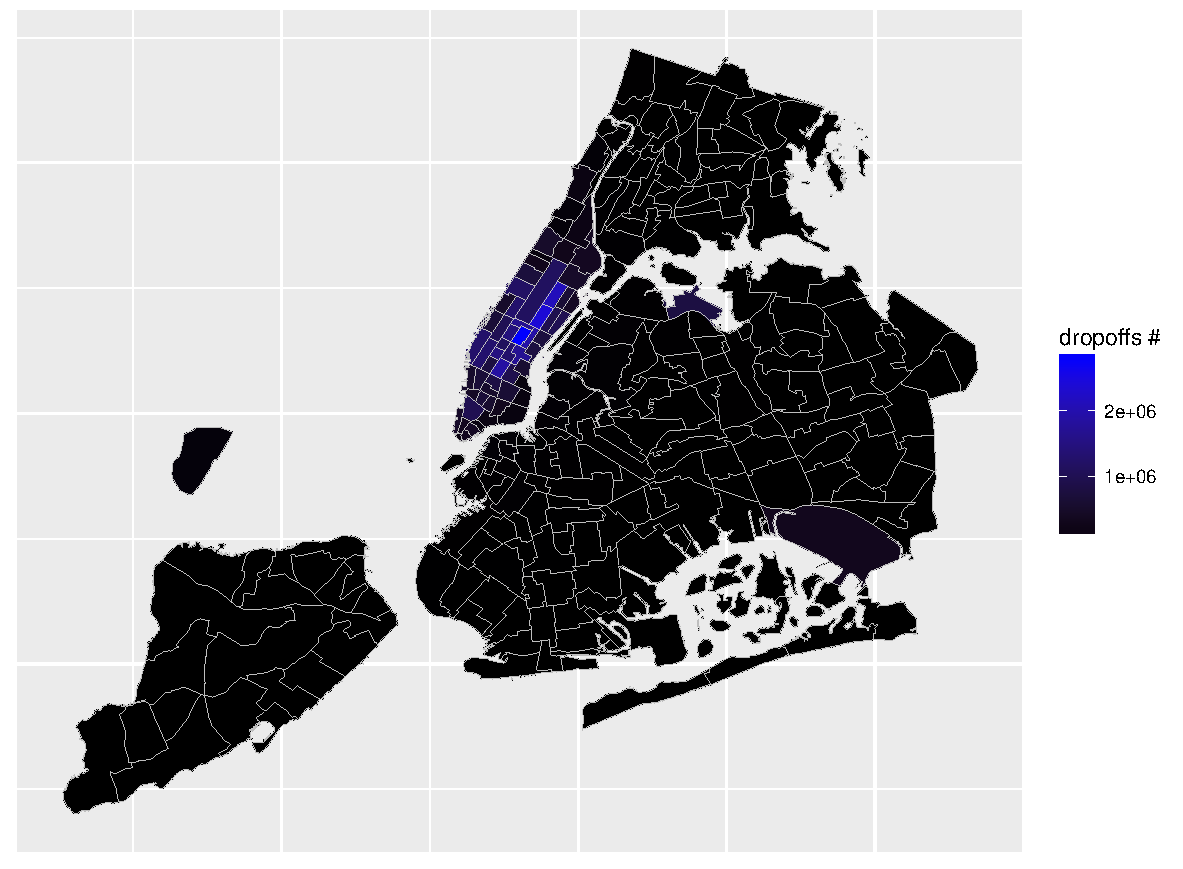
\includegraphics[width=1\columnwidth]{resources/base_plots/manhattan_dropoff_location_id_by_pickup_hour_dist10_map.pdf}}\\
	\subfloat[Dropoff locations at 22]{\label{fig:manhattan33DropoffMap}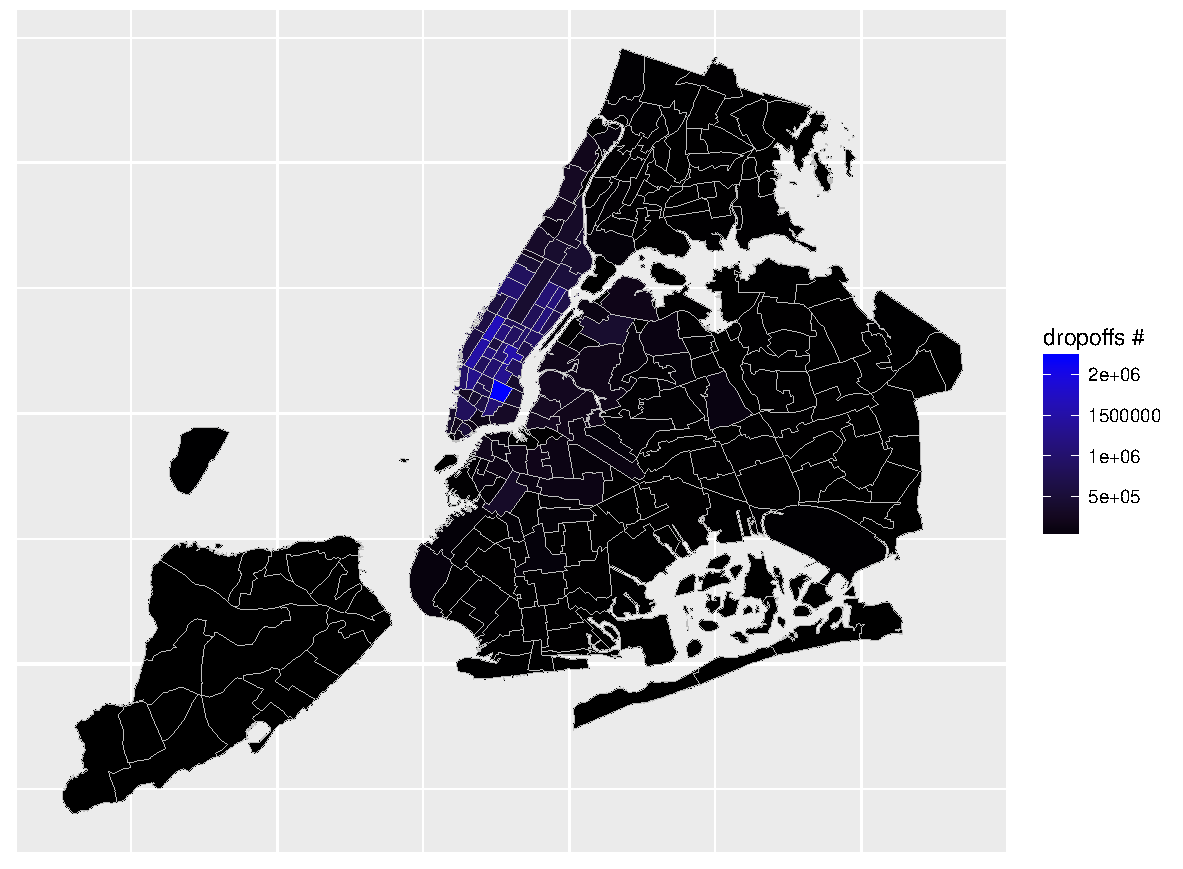
\includegraphics[width=1\columnwidth]{resources/base_plots/manhattan_dropoff_location_id_by_pickup_hour_dist23_map.pdf}}
	\caption{Map in showing the preferred dropoff locations for rides starting inside the Manhattan borough, overall, at 10 and at 23.}
	
\end{figure}

\cref{fig:bronxDropoffMap} depicts the distribution of dropoff locations for pickups happened in the Manhattan borough. Most dropoffs happen within Manhattan itself or in the airports. During the day the most active dropoff zones are those on the South East corner of Central Park, while after 20, most of the dropoffs concentrate in the South West Manhattan area and in East Village. From this fact and from some research on the New York nightlife we infer that this shift is caused by people moving to these zones to experiment the New York nightlife. The fact is cross checked by looking at the locations where most pickups happen at night, which are again South West Manhattan and East Village.

\begin{figure}
	\centering
	\subfloat[Overall dropoff locations (log scale)]{\label{fig:queensDropoffMap}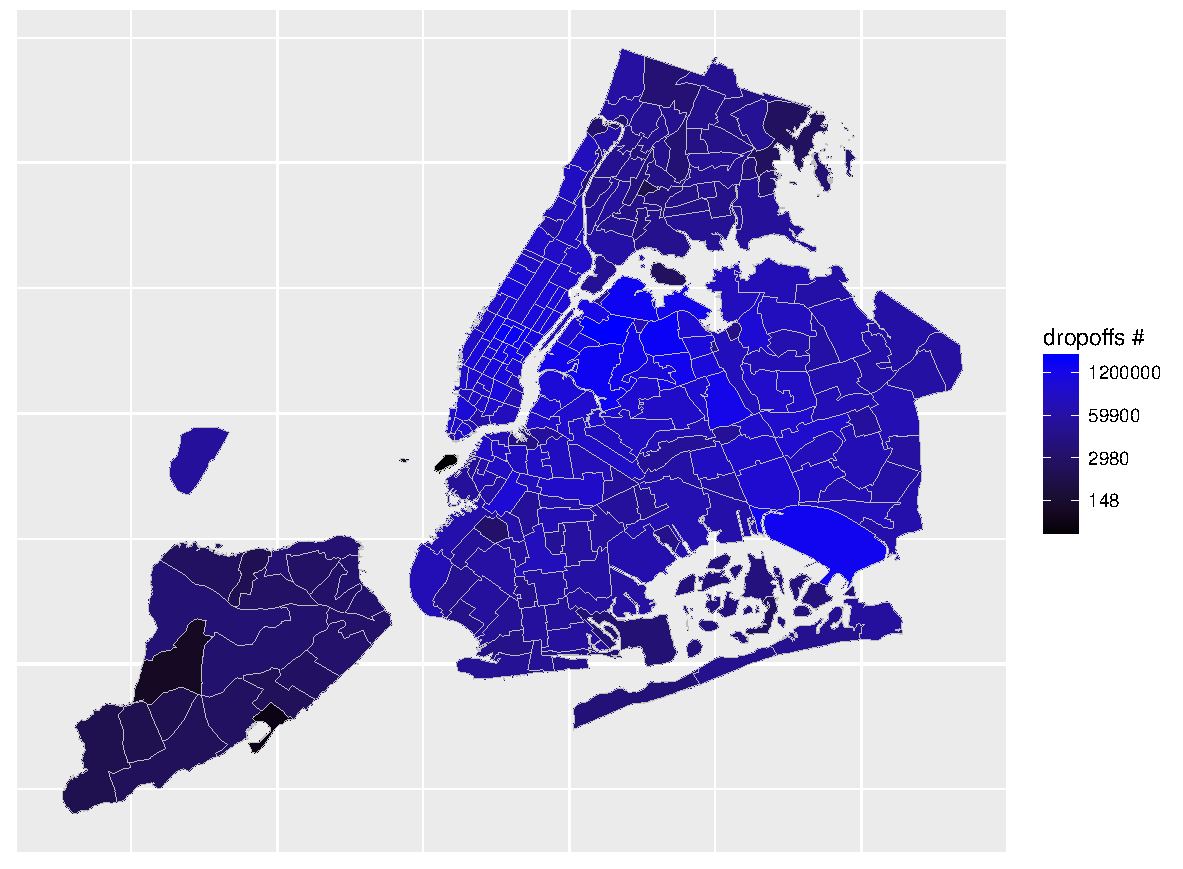
\includegraphics[width=1\columnwidth]{resources/base_plots/queens_dropoff_location_id_dist_map.pdf}}\\
	\subfloat[Dropoff locations at 12]{\label{fig:queensDropoff12Map}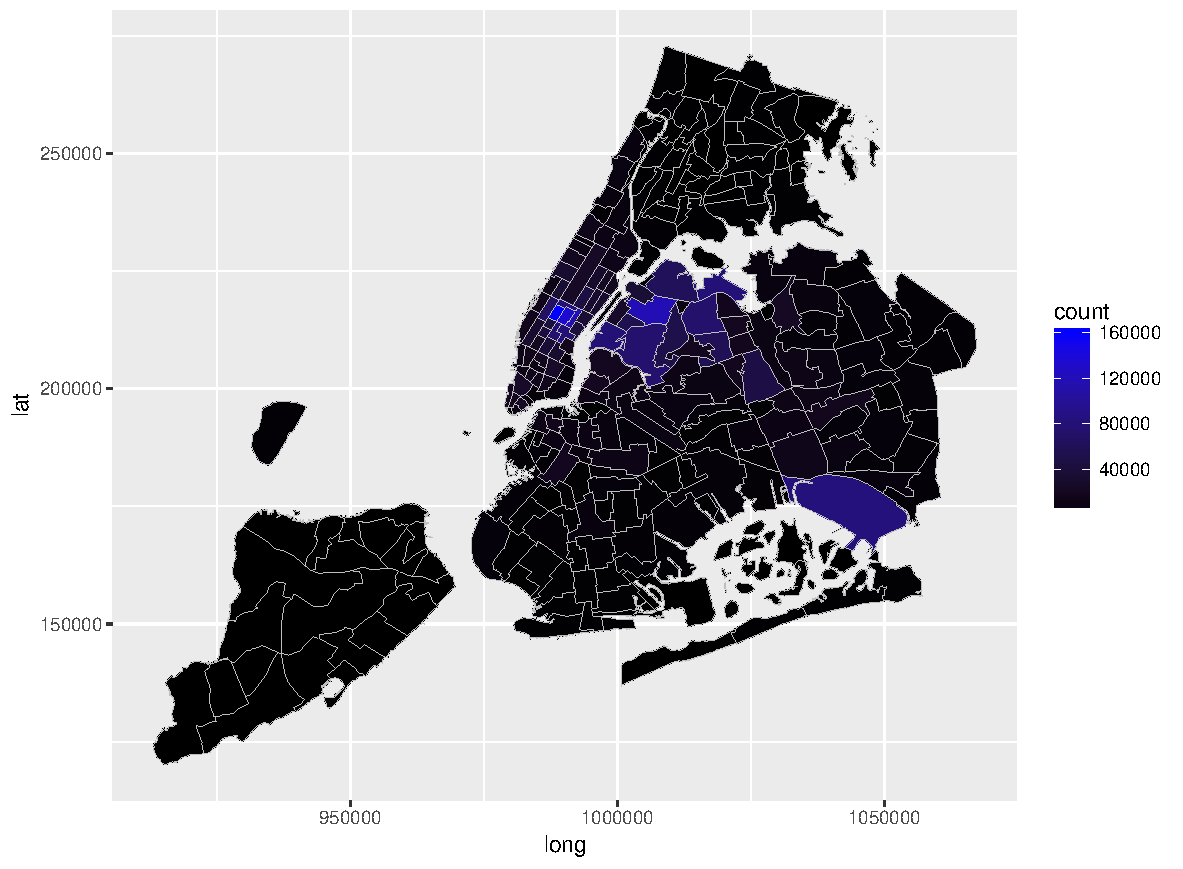
\includegraphics[width=1\columnwidth]{resources/base_plots/queens_dropoff_location_id_by_pickup_hour_dist12_map.pdf}}
	\caption{Map showing the preferred dropoff locations for rides starting inside the Queens borough, overall and at 12. Note how at 12 a consistent part of the traffic goes to the Manhattan district under Central Park. This movement remains constant all day from 7 to 16.}
\end{figure}

\cref{fig:queensDropoffMap} shows the distribution of dropoff locations for pickups happened in the Queens borough. The majority of dropoffs happen in North West Queens, the adjacent part of Manhattan and at the airports. We notice that from 7 to 16 there is a steady movement of people from Queens to the Manhattan districts South of Central Park, similar to that shown in \cref{fig:queensDropoff12Map}. By isolating the airport traffic it can be seen that a part of this phenomenon is caused by trips started at airports that seem to prefer the zones below Central Park as destination.

\begin{figure}
	\centering
	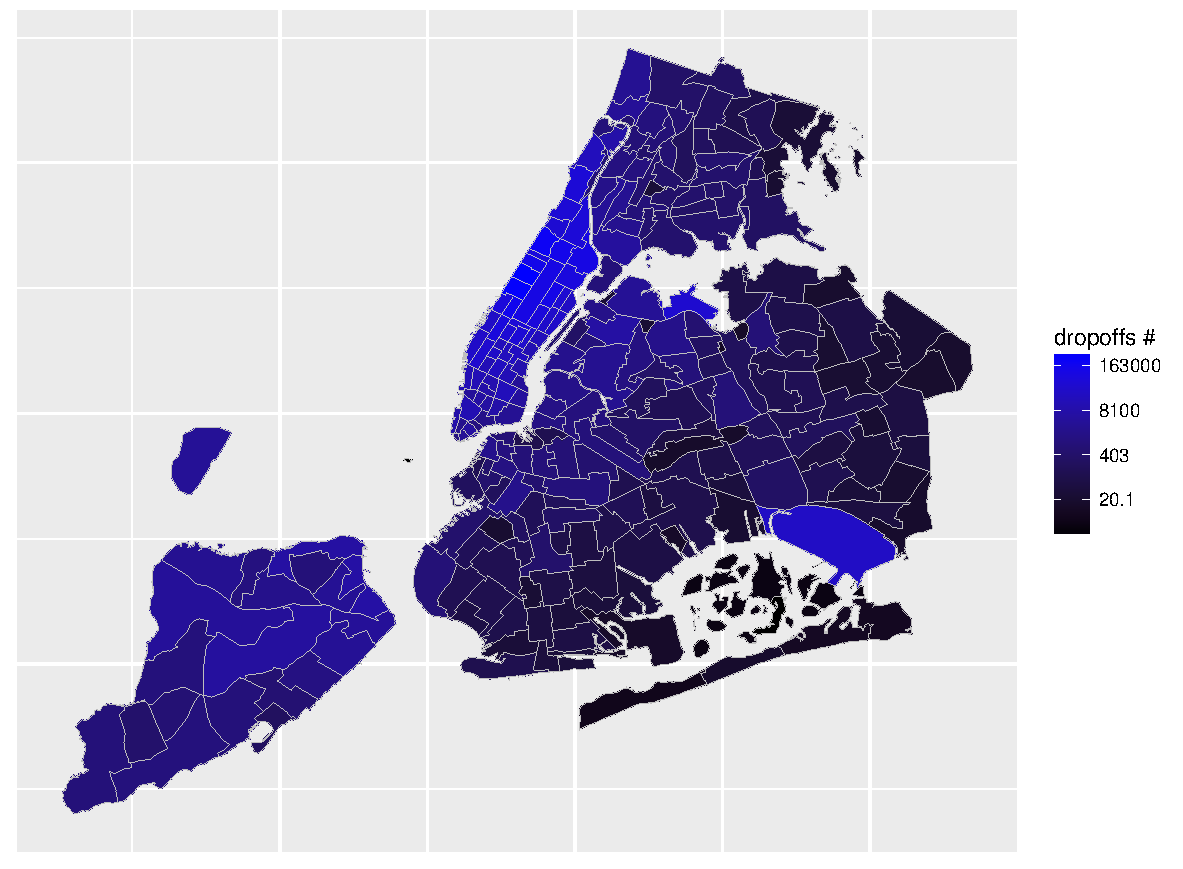
\includegraphics[width=1\columnwidth]{resources/base_plots/staten_island_dropoff_location_id_dist_map.pdf}
	\caption{Map in logarithmic scale showing the preferred dropoff locations for rides starting inside the Staten Island borough.}
	\label{fig:statenIslandDropoffMap}
\end{figure}

\cref{fig:statenIslandDropoffMap} shows the distribution of dropoff locations for pickups happened in the Staten Island borough. This district features an anomalous behavior in that the majority of dropoffs happen in the zones West of Central Park and the airports instead of inside Staten Island itself. This behavior remains constant throughout the whole day.

\section{Yellow vs Green cabs}

A major change in the taxi business was given by the addition of green taxis along with the traditional yellow cabs. In this section we analyze the impact of this introduction and the difference from the yellow taxis.

\begin{figure}
	\centering
	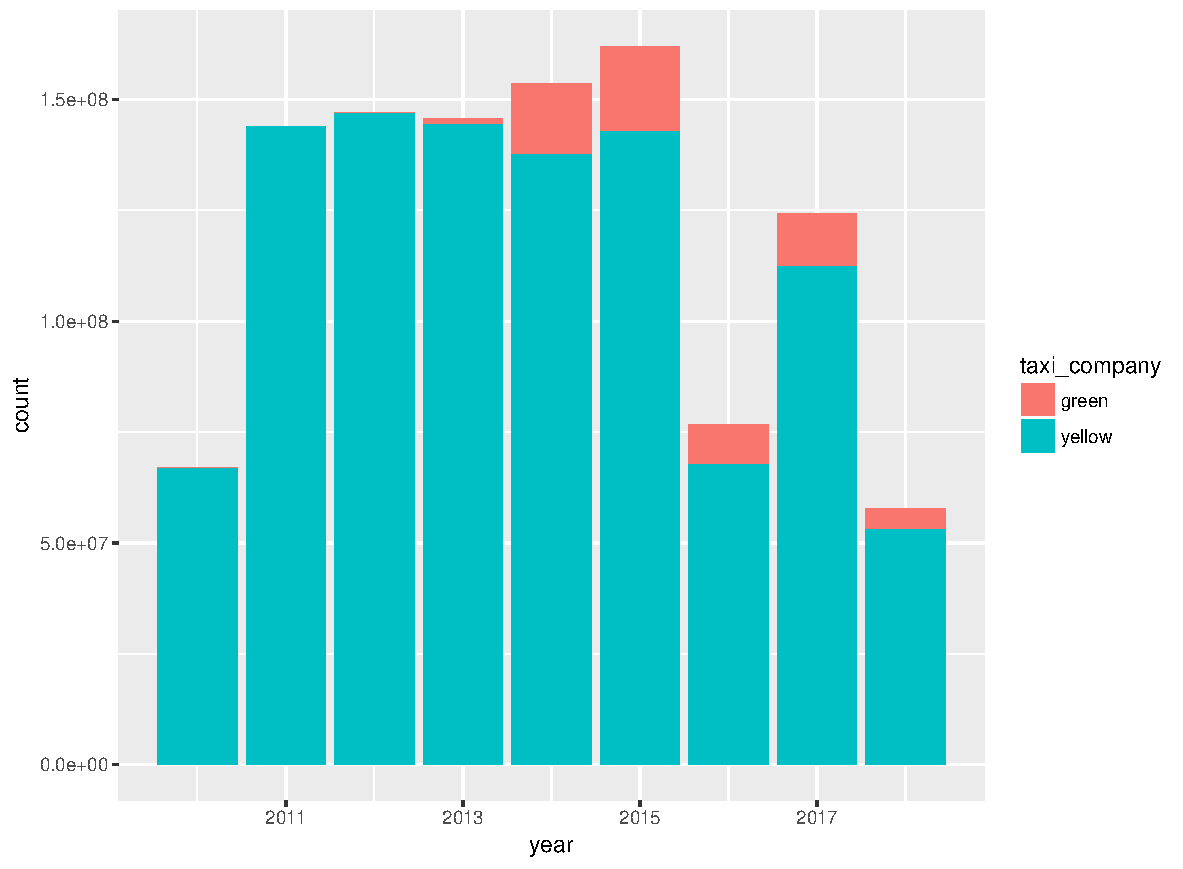
\includegraphics[width=1\columnwidth]{resources/base_plots/travels_by_year_and_company.pdf}
	\caption{Total trips performed each year divided by taxi type. Data for years 2010 and 2016 is missing due to data quality problems, while data for 2018 is only relative for the period January-June.}
	\label{fig:travelsByYearAndCompany}
\end{figure}

\cref{fig:travelsByYearAndCompany} shows the distribution of trips between the companies in the years from 2010 to 2018. We can notice that the introduction of green taxis caused a slight reduction of the trips performed by yellow taxis and from 2015 both types of taxi suffered from a substantial decrease due to the competition of companies such as Uber.

\begin{figure}
	\centering
	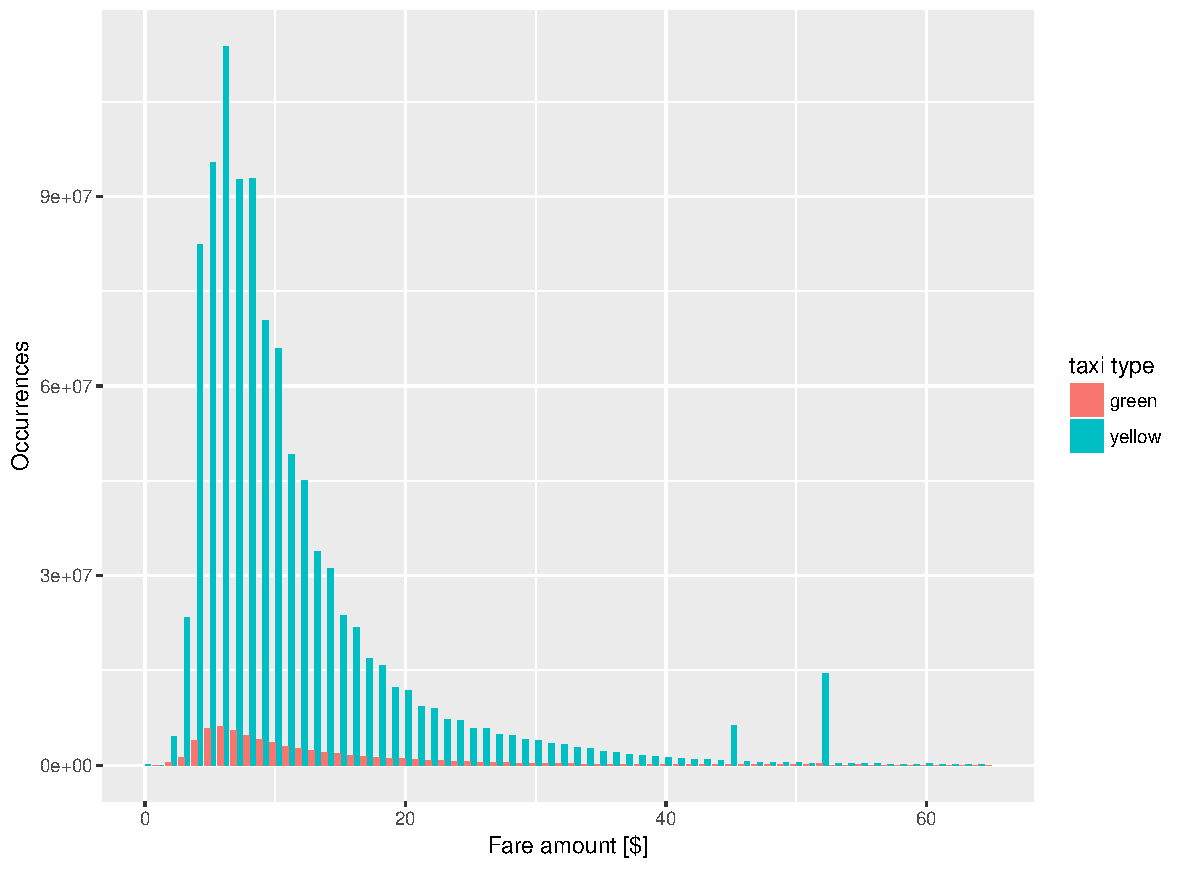
\includegraphics[width=1\columnwidth]{resources/base_plots/fare_amount_by_company_distr.pdf}
	\caption{Fare amount distribution divided by company. 45\$ and 52\$ fares represent special fare rates to the airport.}
	\label{fig:fareAmountByCompany}
\end{figure}

Looking at \cref{fig:fareAmountByCompany}, which compares the distribution of fare amounts, we immediately notice that the curves have similar shape, although the longest and profitable airport trips, the ones with 52\$ fare rate, are almost always performed by yellow cabs. This is expected, since green cabs can only perform dropoffs at the airport and pick up passengers only if the trip is arranged in advance, which is a severe limitation.

\begin{figure}
	\centering
	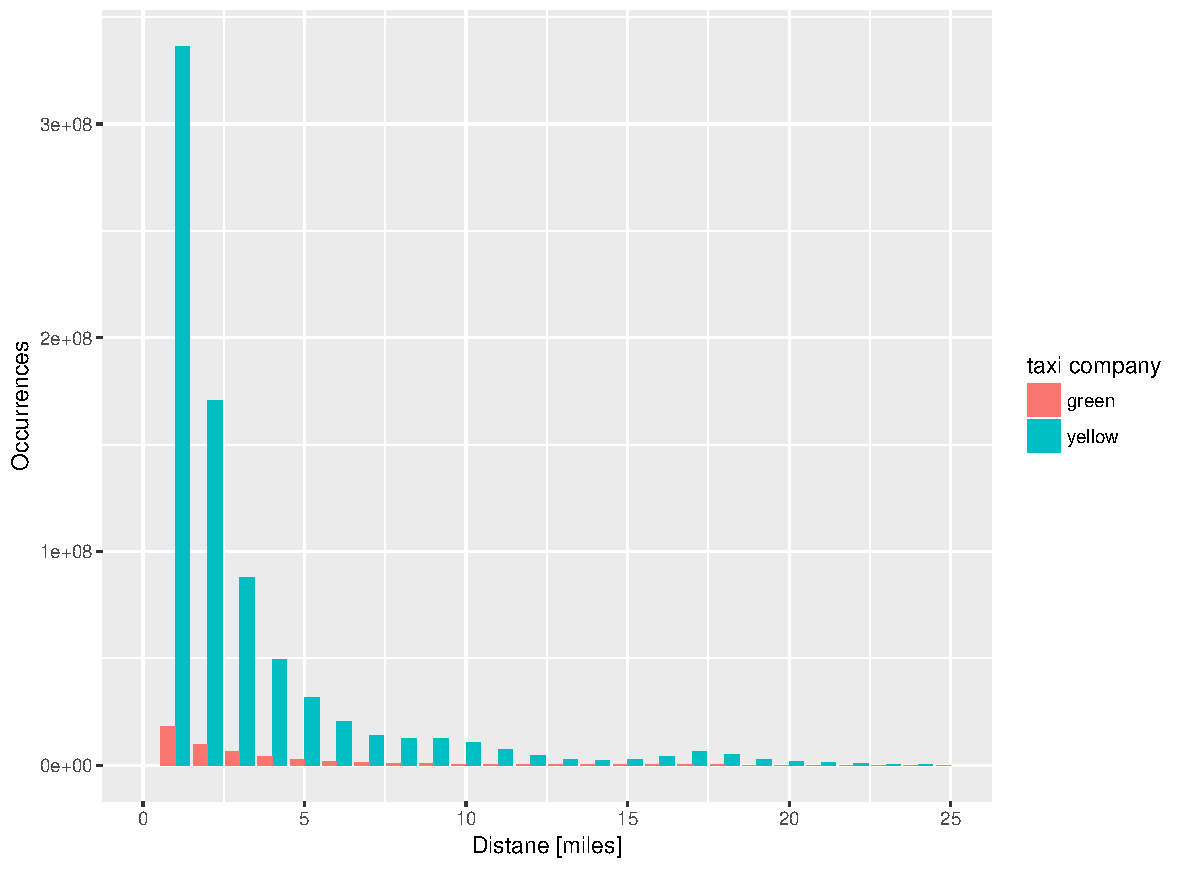
\includegraphics[width=1\columnwidth]{resources/base_plots/trip_distance_by_company_distr.pdf}
	\caption{Trip distance distribution divided by company.}
	\label{fig:tripDistanceByCompany}
\end{figure}

By analyzing \cref{fig:tripDistanceByCompany} we also note that, while the distribution of yellow taxis is trimodal, the distribution for green taxis is not. In particular we notice that green taxis miss the 9 miles and 17 miles mode, which are the trips to the JFK and LaGuardia airports. Trips at LaGuardia airport do not happen often for the same limitations of green taxis explained in the former paragraph.

\begin{figure}
	\centering
	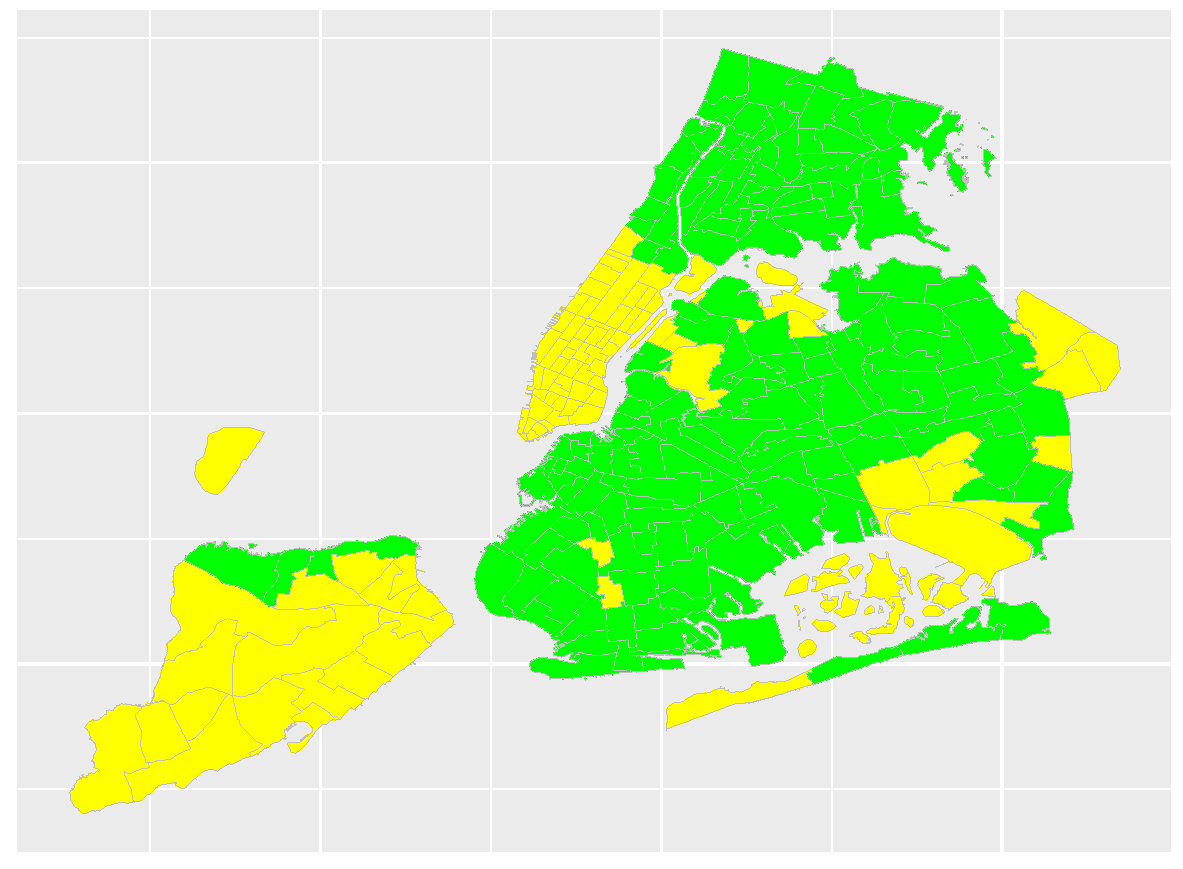
\includegraphics[width=1\columnwidth]{resources/base_plots/pickup_location_by_company_after_2014_distr_difference_map.pdf}
	\caption{Map showing which taxi type preveals in the various zones since year 2014. Yellow zones show where yellow taxis perform the most pickups, green zones represent the ones where green taxis perform more pickups. Notice how Manhattan and the airport zones are prevalently served by yellow taxis.}
	\label{fig:companyDivisionMap}
\end{figure}
\begin{figure}
	\centering
	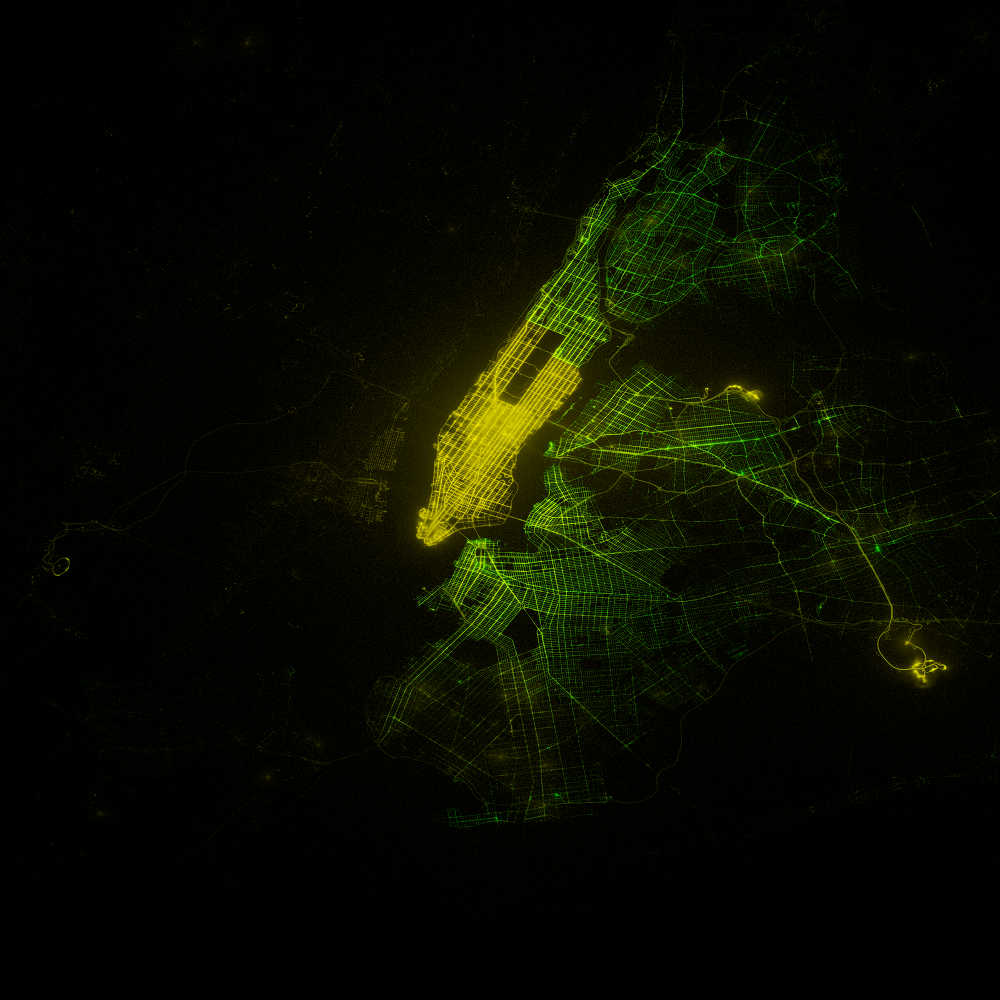
\includegraphics[width=1\columnwidth]{resources/base_plots/yellow_vs_green_pickup.png}
	\caption{Pickup points of yellow and green taxis in their respective color. Notice how Manhattan and the airports feature yellow prevalence, while the other zones feature a green prevalence. For the high resolution version see \cref{sec:shared_folder}}
	\label{fig:companyDivisionImageMap}
\end{figure}

Green taxis were introduced explicitly to help serving the outer boroughs, where it is difficult to find a yellow cab, because they prefer to remain in the profitable Manhattan zone. \cref{fig:companyDivisionMap} shows which taxi type is more popular in the various zones since year 2014. Indeed we can see that green taxis became prevalent in North Manhattan, where they are allowed to pick up passengers, and in every outer borough with the exception of Staten Island and the two airport zones where they are not allowed to perform non arranged pickups. \cref{fig:companyDivisionImageMap} shows an alternative view of the yellow-green taxi presence in New York.

\section{Airport traffic}

Given the relevance of the airport traffic emerged by the previous analysis step, we decide to perform a more thorough analysis of the traffic originated or directed to the three airports. The first remark is that, due to Newark airport not being in a valid taxi zone, the data cleaning phase removed many of the trips to the Newark airport and so data regarding it is not reliable.

\begin{figure}
	\centering
	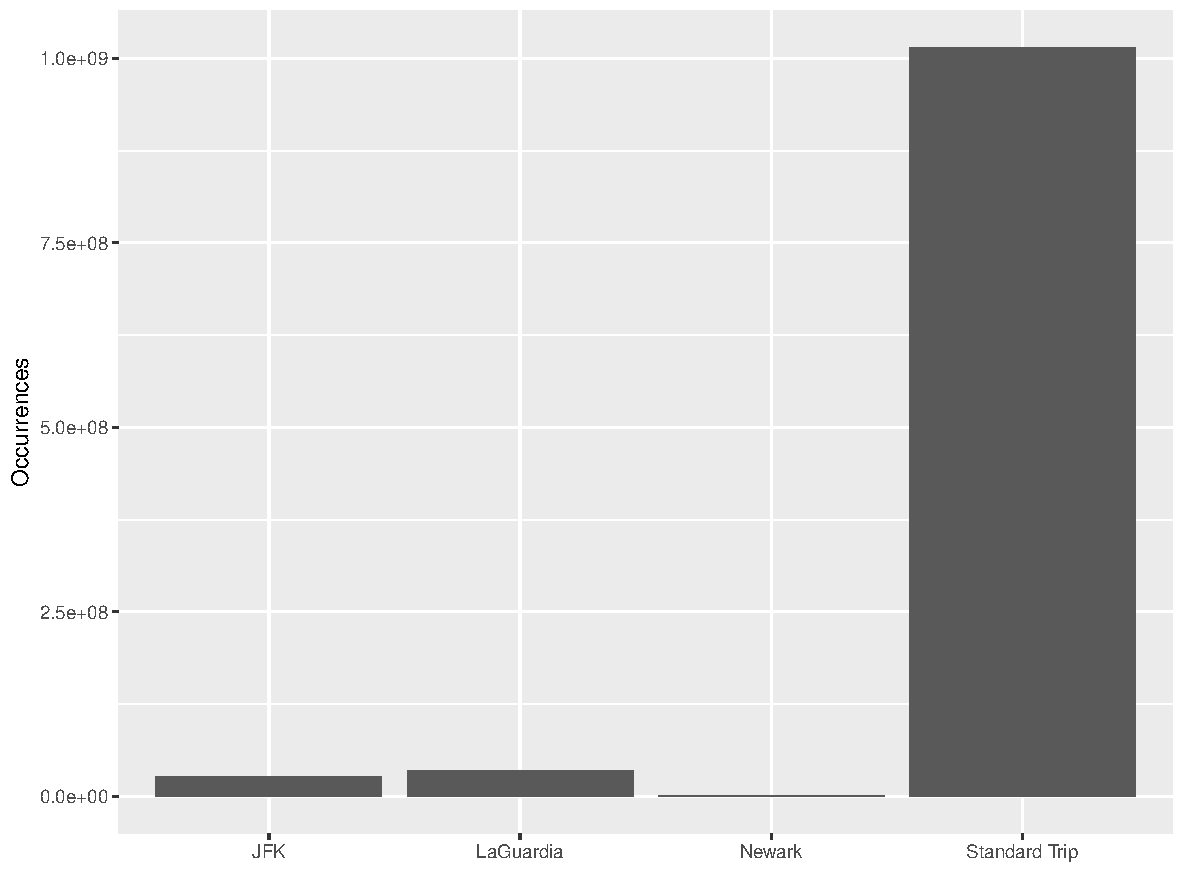
\includegraphics[width=1\columnwidth]{resources/airport/airport_distr.pdf}
	\caption{Total number of trips performed from January 2010 to June 2018 divided by airport. Airport trips make 5.92\% of total taxi trips.}
	\label{fig:airportDistr}
\end{figure}

\begin{figure}
	\centering
	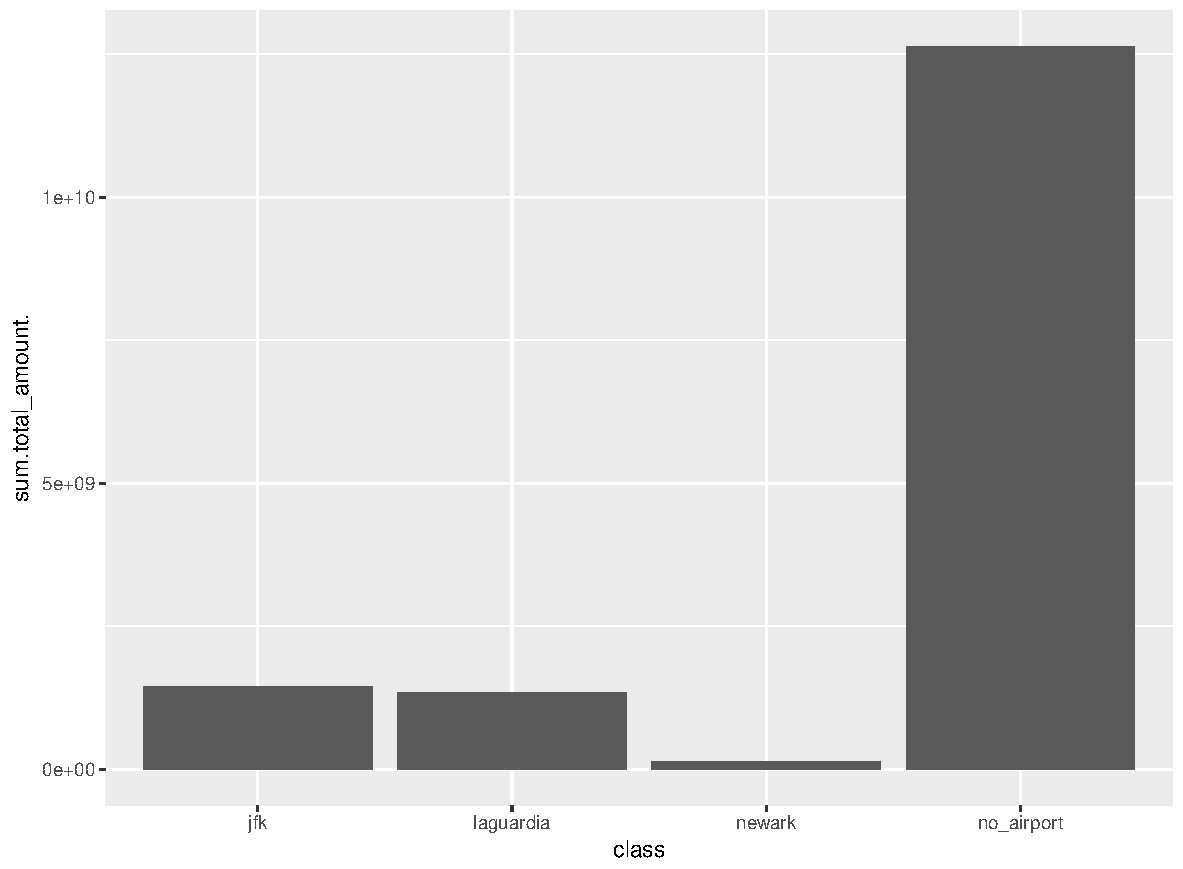
\includegraphics[width=1\columnwidth]{resources/airport/total_amount_by_airport.pdf}
	\caption{Total revenue from January 2010 to June 2018 divided by airport. Airport trips make 18.7\% of total taxi revenue.}
	\label{fig:airportProfitDistr}
\end{figure}

\begin{figure}
	\centering
	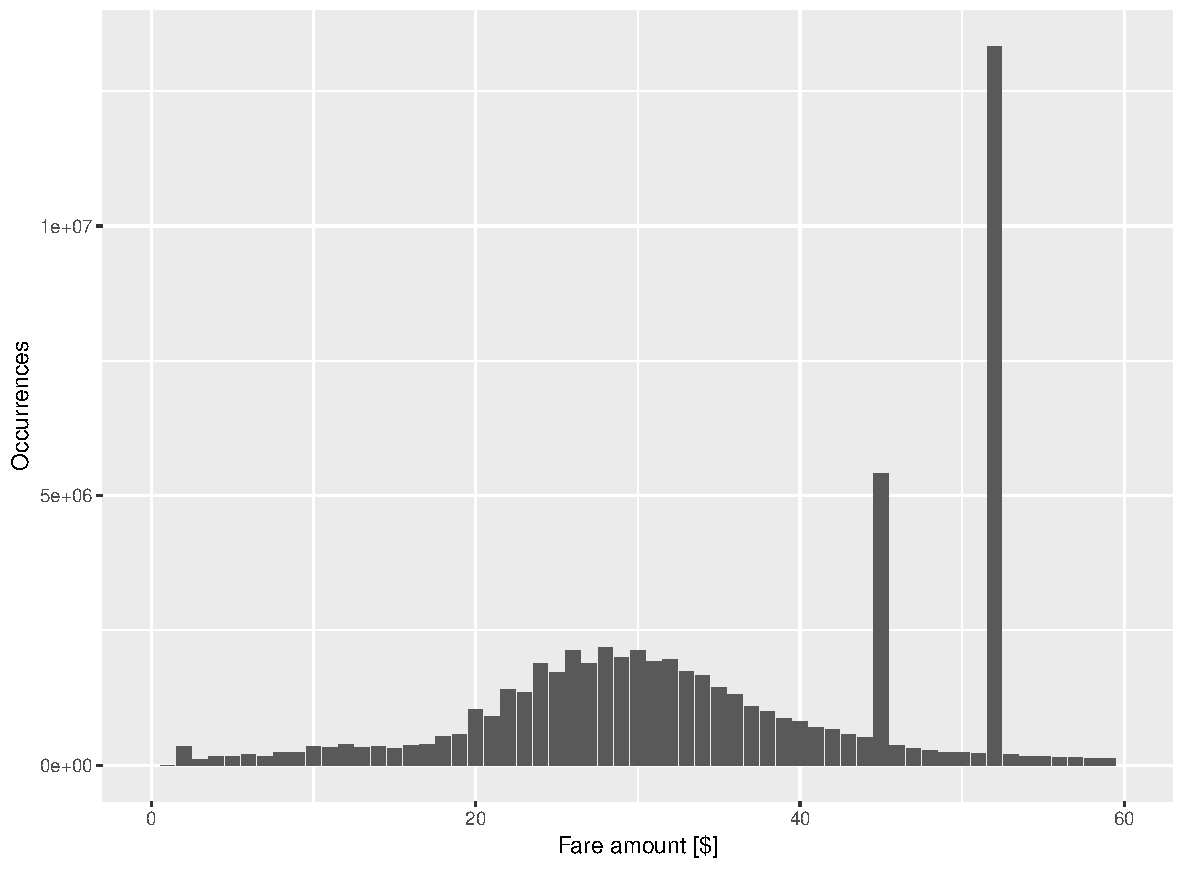
\includegraphics[width=1\columnwidth]{resources/airport/fare_amount_distr.pdf}
	\caption{Distribution of fare amount. Notice the mode at ~30\$ corresponding to trips to LaGuardia airport and the 45\$ and 52\$ flat rate amounts corresponding to trips to JFK from Manhattan. The right heavy tail is given by trips to the JFK from outside Manhattan that are not subject to the flat rate.}
	\label{fig:airportFareAmount}
\end{figure}

We first notice from \cref{fig:airportDistr} that airport trips make a relatively small 5.92\% of the total number of taxi trips. Despite that, as \cref{fig:airportProfitDistr} shows, they are a major stream of revenue for taxis due to the very high cost per trip, making 18.7\% of their profits. In fact, by looking at the fare rate distribution in \cref{fig:airportFareAmount}, and comparing it with \cref{fig:fareAmountDistr} we can see that fare amounts for LaGuardia averages around 30\$, fare amounts towards JFK have a fixed fare rate of 52\$ (45\$ before fare rate revision operated in 2012), while the in majority of common taxi trips the fare amounts are below 10\$. It it thus not surprising that yellow taxi owners fought for forbidding green taxis to pick up passengers at airports.

\begin{figure}
	\centering
	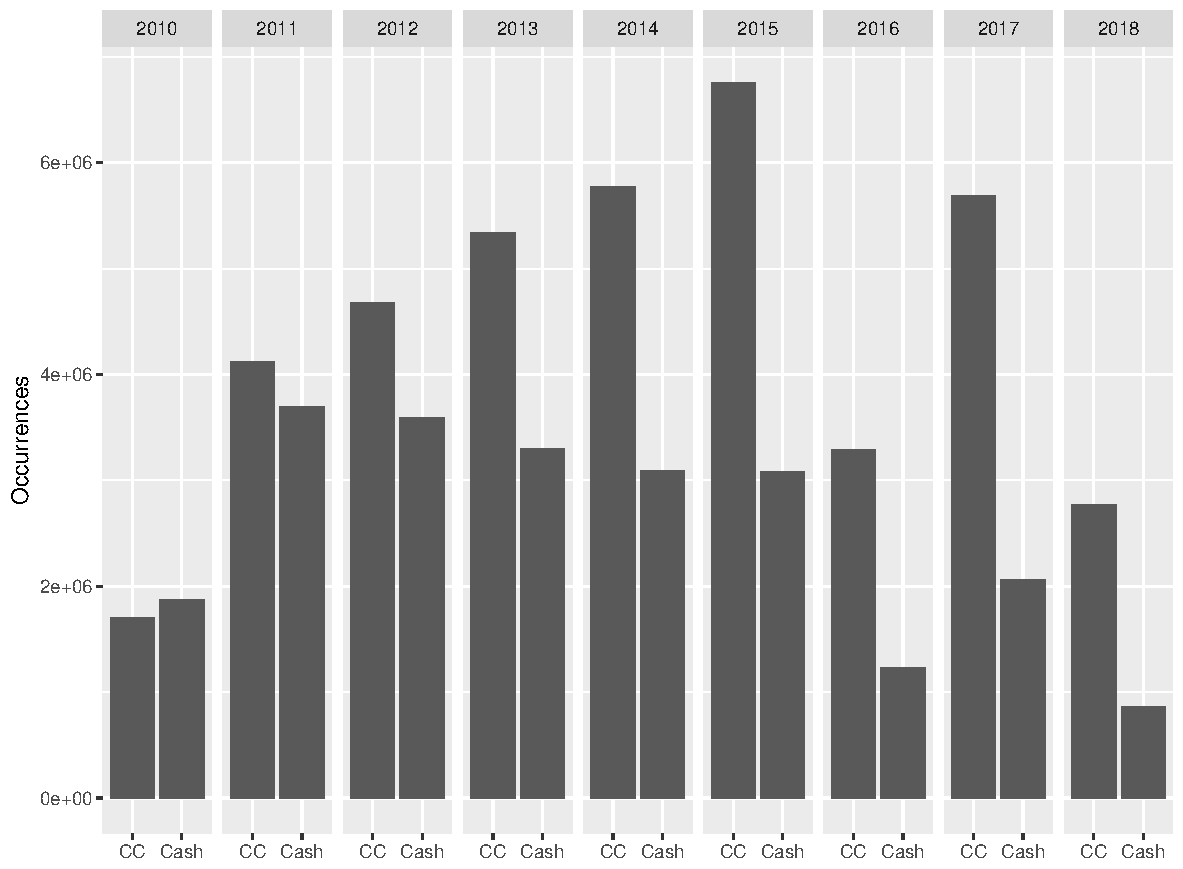
\includegraphics[width=1\columnwidth]{resources/airport/payment_type_distr.pdf}
	\caption{Distribution of payment methods from 2010 to 2018. Notice how already from 2011 credit card payments make for the majority of payments. The higher percentage of credit card payments is probably given by the high cost of airport trips.}
	\label{fig:airportPaymentType}
\end{figure}

By looking at the distribution of payment types in \cref{fig:airportPaymentType} it is also interesting to notice that the percentage of people paying with credit cards is higher than its percentage in common taxi trips shown in \cref{fig:paymentTypeByYear}. This is probably due to the higher total amounts.

\begin{figure}
	\centering
	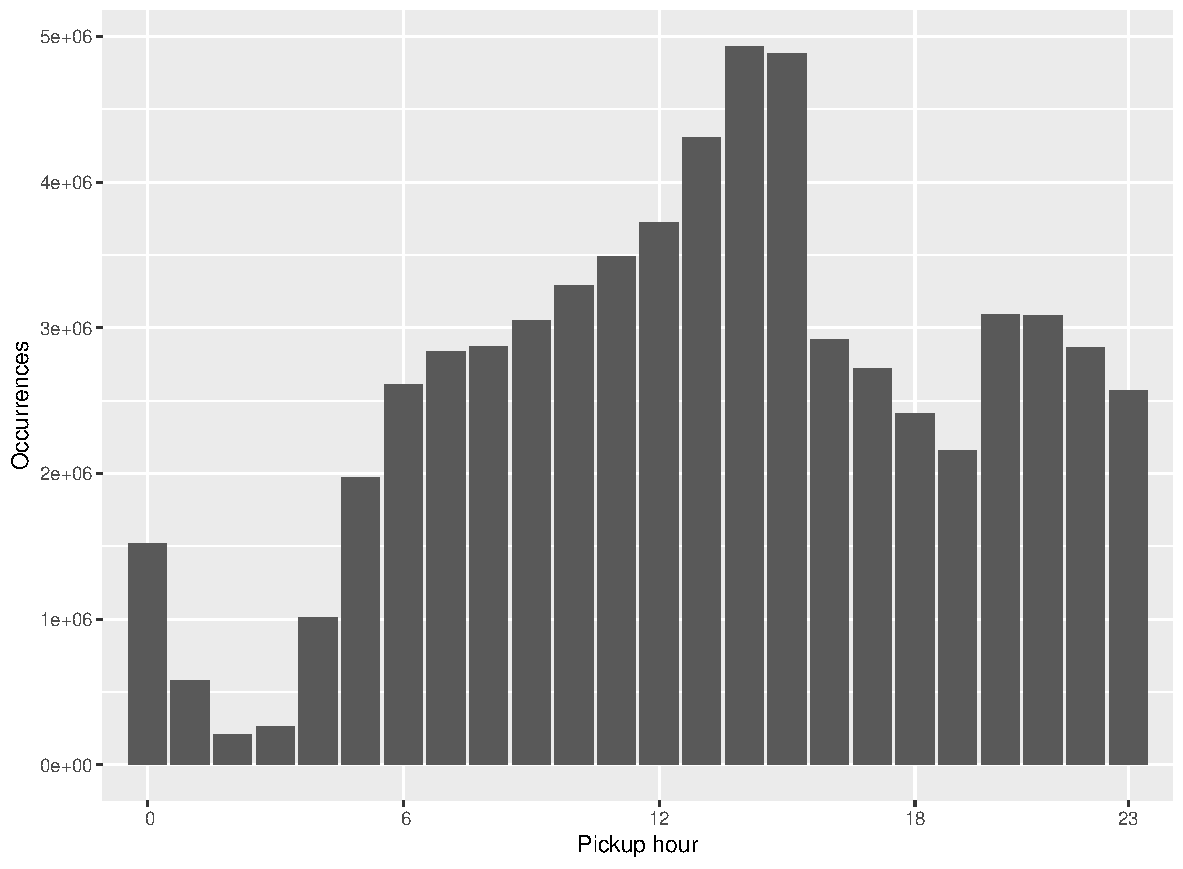
\includegraphics[width=1\columnwidth]{resources/airport/pickup_hour_dist.pdf}
	\caption{Number of pickups divided by hour. The peak activity is reached at 14 and is almost absent from 24 to 5.}
	\label{fig:airportPickupHourDistr}
\end{figure}


From \cref{fig:airportPickupHourDistr} we can look at the number of trips as a function of pickup hour. This can be seen as a rough indicator of airport activities through the day. We notice that activity starts at about 5, then peaks at 14 and slowly decreases until 24, after which activity is enormously reduced. By comparing it with standard taxi activity shown in \cref{fig:pickupHourDist} we can see that airport traffic completely lacks the peak experimented at 20 and reinforces the hypothesis that the peak at 20 in normal traffic is caused by nightlife.

\begin{figure}
	\centering
	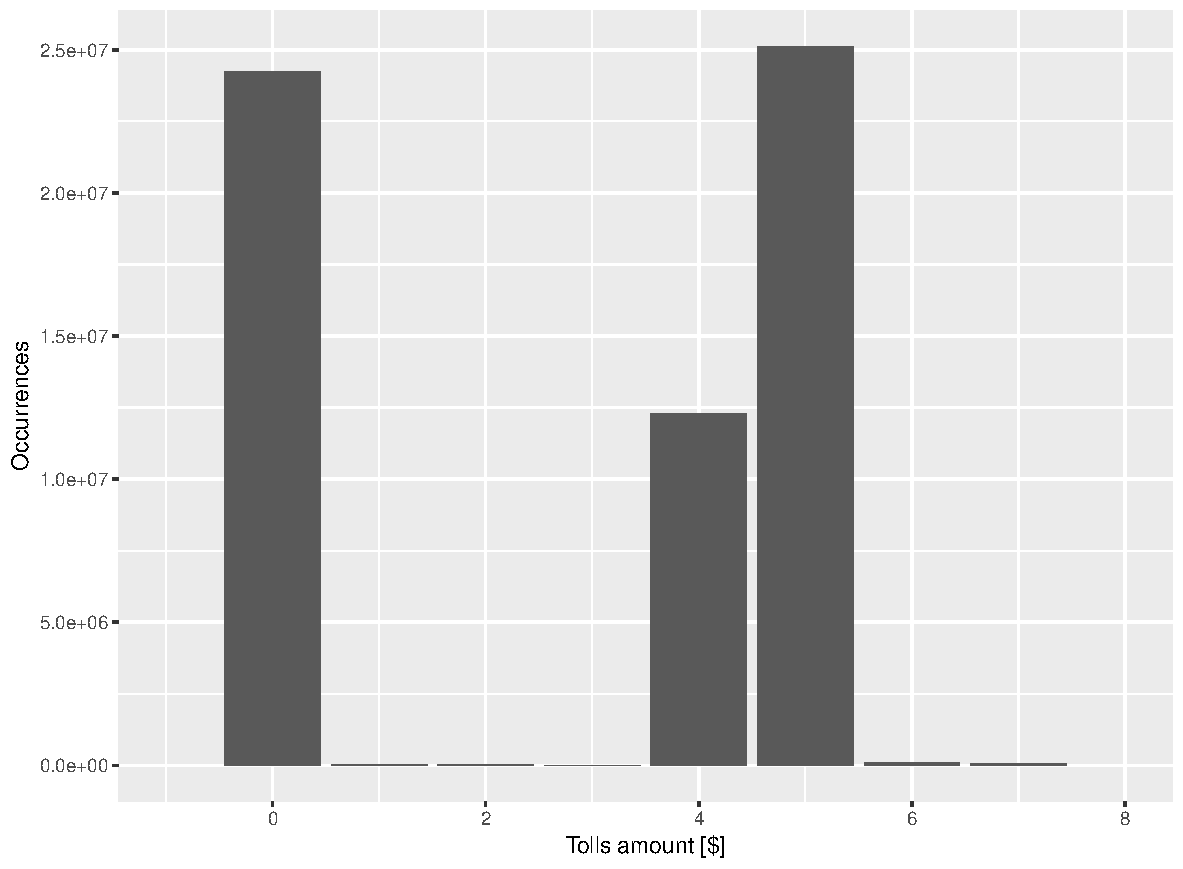
\includegraphics[width=1\columnwidth]{resources/airport/tolls_amount_distr.pdf}
	\caption{Distribution of tolls amount. Notice how the number of trips subject to tolls are the majority.}
	\label{fig:airportTollsAmount}
\end{figure}

As a last remark, by looking at the distribution of tolls amount in \cref{fig:airportTollsAmount}, we notice that the number of trips subject to tolls is the majority with respect to the total number of trips. By comparing it with \cref{fig:tollsAmountDistr} we see that airport trips are responsible for the majority of trips that were subject to tolls.

\section{Conclusions}

In this paper we presented an overview of many aspects of the NYC taxi service, starting from an high level description and later proceeding more in depth in some selected topics. We highlighted some of the service's problems such as the concentration of yellow taxis in Manhattan and the airports which creates a difficulty for passengers of outer boroughs to find hails despite the introduction of green taxis, the increasing trend of fare amounts and the problematic level of city traffic which causes very low average moving speeds. It is our opinion that these and other factors such as the historically inadequate number of yellow taxi Medallions and problems in the public transport infrastructure play an important role in the success of ride hailing applications such as Uber which are experiencing huge gains in popularity, threatening the position of the taxi service.

Further topics of interest which have not been analyzed at the moment include a study of weekend traffic which seems to have peculiar characteristics, study of the effects of weather events on the taxi service, studies regarding the popularity of local businesses such as bars, clubs and pubs in the different zones of the city or a series of studies regarding the movement of employees of certain companies such as Accenture, the Goldman Sachs Group or American Express which could give a picture of where the wealthiest part of the population lives in the city.

%
% The following two commands are all you need in the
% initial runs of your .tex file to
% produce the bibliography for the citations in your paper.
\bibliographystyle{abbrv}
\bibliography{main}


\balancecolumns
\appendix
%Appendix A
\section{Files and Script Execution}
\label{sec:shared_folder}

This appendix describes the contents of the shared Google Drive directory and describes what is needed in order to run the scripts. The directory is composed of the following parts

\begin{itemize}
	\item \texttt{src} folder, containing the Python and R sources
	\item \texttt{report} folder, containing the files used to produce the report
	\item \texttt{data} folder, containing the dataset and some helper files for faster dataset construction
	\item \texttt{plots} folder, containing all the obtained plots and the high resolution version of images shown in the report
	\item \texttt{spark\_results} folder, containing all the \texttt{.csv} results produced by Spark
\end{itemize}

The src folder is composed of the following parts:

\begin{itemize}
	\item Spark Python files in the root directory
	\item R scripts for the production of plots and additional data analysis in the R folder
	\item Docs and additional material in the docs directory
\end{itemize}

The dataset folder contains the following elements:

\begin{itemize}
	\item \texttt{tar\_gz\_dataset} folder, containing the compressed dataset from 2010 to 2018 for yellow and green taxis 
	\item \texttt{clustering\_model.model} precomputed clustering model
	\item \texttt{clustered\_dataset.parquet} precomputed dataset, ready for the analysis
	\item \texttt{daily\_trips\_by\_geography.csv} public archive from toddwschneider containing aggregate information about for hire vehicle operations in New York City
\end{itemize}

In order to obtain from scratch the results presented in the report, the following steps must be carried out in this order, but you may use intermediate results to speed up the process if you wish to, as described later in this section:

\begin{itemize}
	\item Install Python packages \texttt{matplotlib}, \texttt{numpy}, \texttt{pandas}, \texttt{networkx}, \texttt{fiona}, \texttt{shapely}.
	\item Import the compressed .tar.gz dataset in your cluster infrastructure and convert it in parquet format executing the gz\_to\_parquet\_main.py script. The script needs to be configured as described in its header.
	\item Convert the different dataset years into a dataset with common schema using the \path{common_schema_conversion_main.py} script. The script needs to be configured as described in its header. In particular you need to ensure that the shapefile in the docs folder is available to the main script. Having the \path{lookup_matrix_1000_3.npy} precomputed lookup matrix in the same folder as the python script avoids its recalculation.
	\item Perform data cleaning by executing \path{data_cleaning_main.py} in order to produce the cleaned dataset. Follow the instruction in the script header to configure it before execution.
	\item Perform clustering. The full clustering procedure is the longest and most expensive part of the processing. For this reason we provide the precomputed \path{clustering_model.model} precomputed clustering model along with the dataset. If you insert it in the dataset folder you can comment the lines in the code performing clustering and model saving and direct apply the clustering model to your dataset, producing the clustered dataset. You may also skip the passages until this point by obtaining the \path{clustered_dataset.parquet} dataset from the Google Drive folder. Please refer to the file header to correctly configure your script. If you wish to execute the complete clustering procedure, you may execute the script directly after the required parameters are inserted without commenting out portions of the code.
	\item Obtain the main data statistics by executing \path{data_statistics_main.py}. Please refer to the header file for correct script configuration. The results in form of .csv files can be subsequently used by the R scripts.
	\item Obtain the clustered data statistics by executing the same script, but setting \texttt{clustered\_analysis} to True. Remember to save the results in a different folder in order to be able to import them in R more easily in later steps.
	\item Obtain the airport statistics by executing \path{airport_data_statistics_main.py}. Please refer to the header file for correct script configuration.
	\item (Optional) Execute \path{data_imaging_main.py} in order to obtain plots such as the one of \cref{fig:companyDivisionImageMap}.
	\item (Optional) Execute \path{graph_building_main.py} in order to obtain an interactive graph visualization of the taxi zones.
	\item Install R packages \texttt{ggplot2}, \texttt{RColorBrewer},\texttt{rgdal}, \texttt{ggmap}
	\item Configure and execute \texttt{R/main.R} in order to obtain the first set of plots. In particular the script needs to be given the location of the .csv files obtained during the main analysis step.
	\item Configure and execute \path{R/airport_main.R} in order to obtain the first set of plots. In particular the script needs to be given the location of the .csv files obtained during the airport analysis step.
	\item Configure and execute \path{R/clustering_main.R} in order to obtain the first set of plots. In particular the script needs to be given the location of the .csv files obtained during the clustered analysis step.
\end{itemize}

It may be possible that some other minor steps or slight modification to the code (such as specifying file access protocols \path{hdfs:\\} instead of \path{file:\\}) are required in order to completely run the code on the system of the reader.

If you are interested only in seeing the result \texttt{.csv} files or in running the R scripts to produce the plots you can avoid running Spark entirely and use the \texttt{stats.zip}, \texttt{clustered\_stats.zip} and \texttt{airport\_stats.zip} archives available in the Google Drive folder to obtain the results of Spark elaborations. If you are interested only in seeing the plots you can download the corresponding zip archives from the Google Drive folder.

If you are interested in visualizing the interactive graph, download the \texttt{traffic\_graph.zip} contained in the \texttt{plots} directory of the Google Drive folder, extract the content of the zip in an arbitrary directory, open the \texttt{traffic\_graph} directory, open the \texttt{web\_session} directory and open the \texttt{index.html} file. A web page displaying the interactive version of the graph will be opened. If you are interested in visualizing the legend, open the file \texttt{legend.png} in the same folder.

















\end{document}
